%!TEX root = tfg.tex
\chapter{Resultados obtenidos}

\begin{quotation}[Físico]{Lord Kelvin (1824--1907)}
Lo que no se define no se puede medir. Lo que no se mide no se puede mejorar.
\end{quotation}

\begin{abstract}
Este capítulo presenta y analiza los resultados de los experimentos de navegación realizados con las cuatro configuraciones evaluadas: Dijkstra con y sin suavizado, y A* con y sin suavizado. Los resultados se organizan en dos bloques: métricas estáticas, obtenidas sobre la trayectoria planificada sin ejecución real, y métricas dinámicas, obtenidas durante la navegación real del robot hasta el objetivo más complejo del entorno de simulación.
\end{abstract}

\section{Resultados estáticos}

Las métricas estáticas se obtienen a partir de la trayectoria planificada por NavFn para cada uno de los cuatro objetivos de navegación, sin que el robot se desplace físicamente. Permiten comparar los algoritmos en términos de calidad geométrica del plan: tiempo de cómputo, longitud, suavidad y curvatura.

\subsection{Tiempo de planificación y número de waypoints}

La figura~\ref{fig:waypoints_plantime} muestra la relación entre el número de waypoints del plan y el tiempo de planificación para las cuatro configuraciones evaluadas.

\begin{figure}[H]
    \centering
    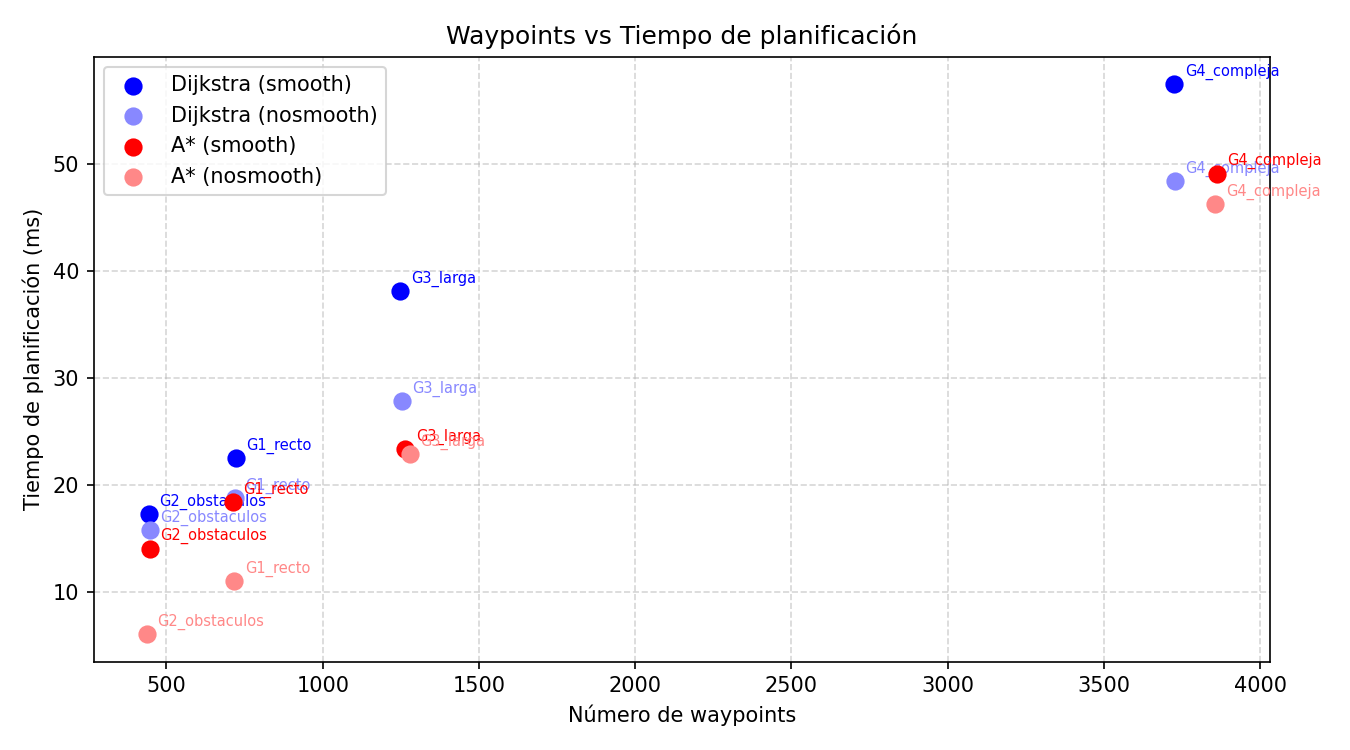
\includegraphics[width=0.9\textwidth]{figures/plots/static/1_waypoints_vs_plantime}
    \caption{Waypoints vs tiempo de planificación para los cuatro objetivos y configuraciones.}
    \label{fig:waypoints_plantime}
\end{figure}

Se observa una correlación clara entre el número de waypoints y el tiempo de planificación: los objetivos más complejos generan planes más largos y tardan más en calcularse. El objetivo más exigente, \texttt{goal4\_compleja}, produce planes de aproximadamente 3.700--3.860 waypoints y tiempos de planificación de entre 46 y 57 ms, mientras que los objetivos más sencillos se resuelven en menos de 25 ms con menos de 800 waypoints.

En cuanto a las diferencias entre algoritmos, A* nosmooth es consistentemente el más rápido: 10,9 ms en \texttt{goal1\_recto} y 46,2 ms en \texttt{goal4\_compleja}. Dijkstra smooth es el más lento, con 22,5 ms y 57,4 ms respectivamente. El overhead del suavizado es apreciable en Dijkstra (entre 3 y 9 ms por objetivo), mientras que en A* la diferencia entre smooth y nosmooth es menor (inferior a 3 ms en todos los objetivos salvo \texttt{goal2\_obstaculos}, donde el suavizado añade 8 ms).

\subsection{Irregularidad de la trayectoria}

Las figuras~\ref{fig:smoothness_dijkstra}, \ref{fig:smoothness_astar} y \ref{fig:smoothness_all} muestran la irregularidad de la trayectoria para cada objetivo y configuración, medida como el cambio de ángulo en valor absoluto acumulado en radianes. Es decir, si el robot gira 90º a la derecha y luego, 90º a la izquierda, la irregularidad sería 180º.

\begin{figure}[H]
    \centering
    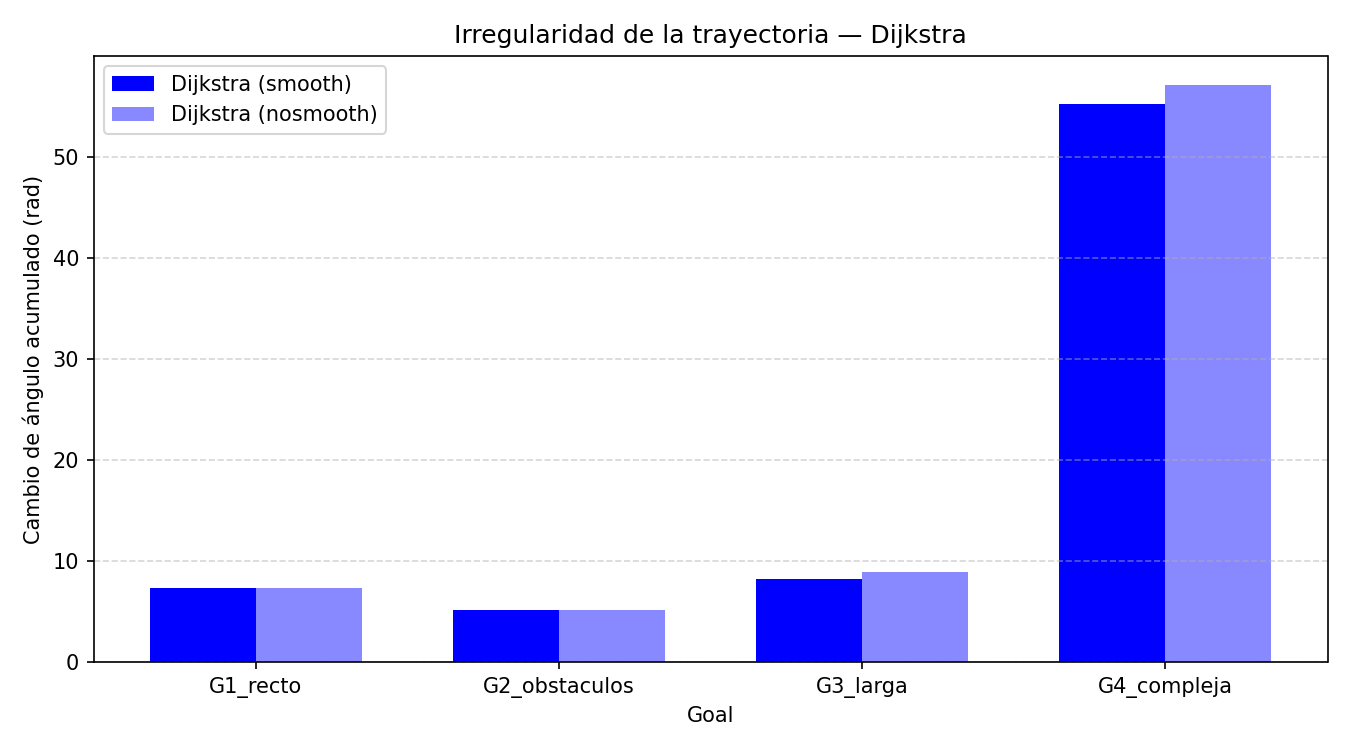
\includegraphics[width=0.85\textwidth]{figures/plots/static/2_smoothness_dijkstra}
    \caption{Irregularidad de la trayectoria — Dijkstra con y sin suavizado.}
    \label{fig:smoothness_dijkstra}
\end{figure}

\begin{figure}[H]
    \centering
    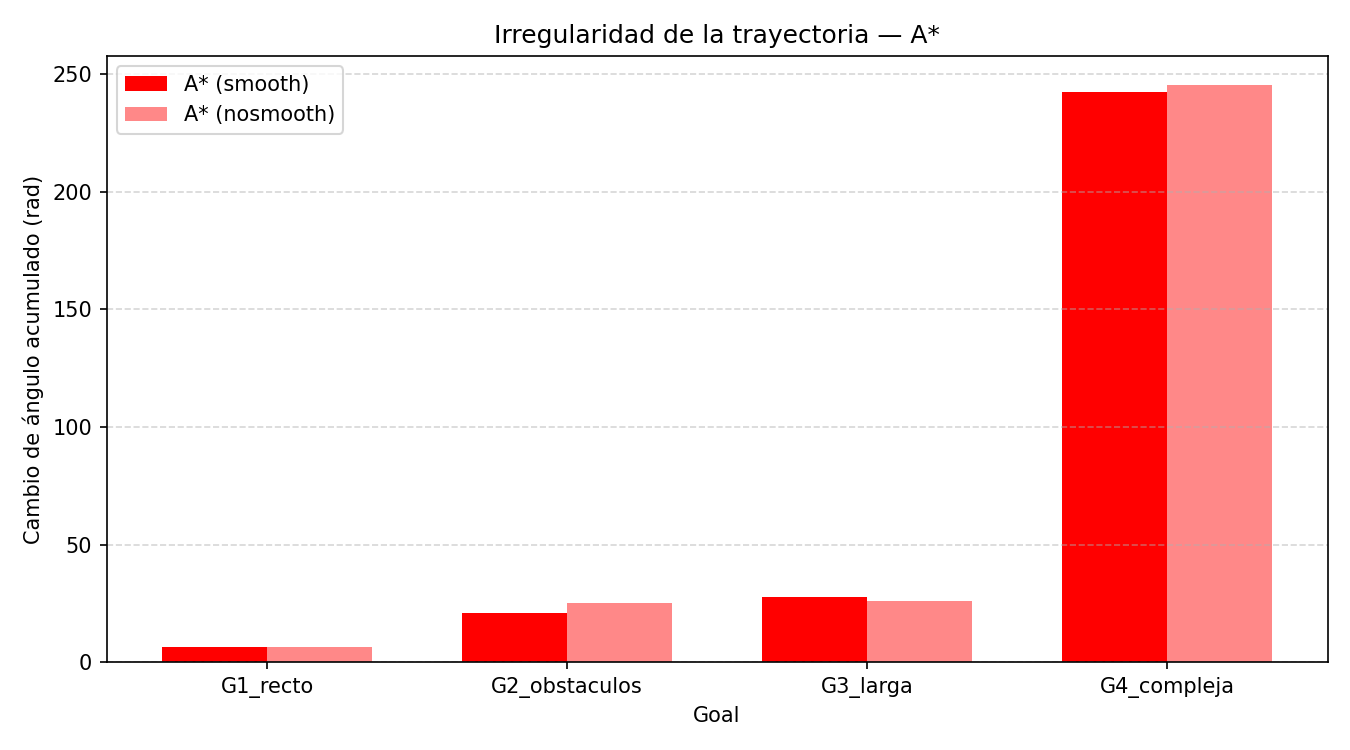
\includegraphics[width=0.85\textwidth]{figures/plots/static/3_smoothness_astar}
    \caption{Irregularidad de la trayectoria — A* con y sin suavizado.}
    \label{fig:smoothness_astar}
\end{figure}

\begin{figure}[H]
    \centering
    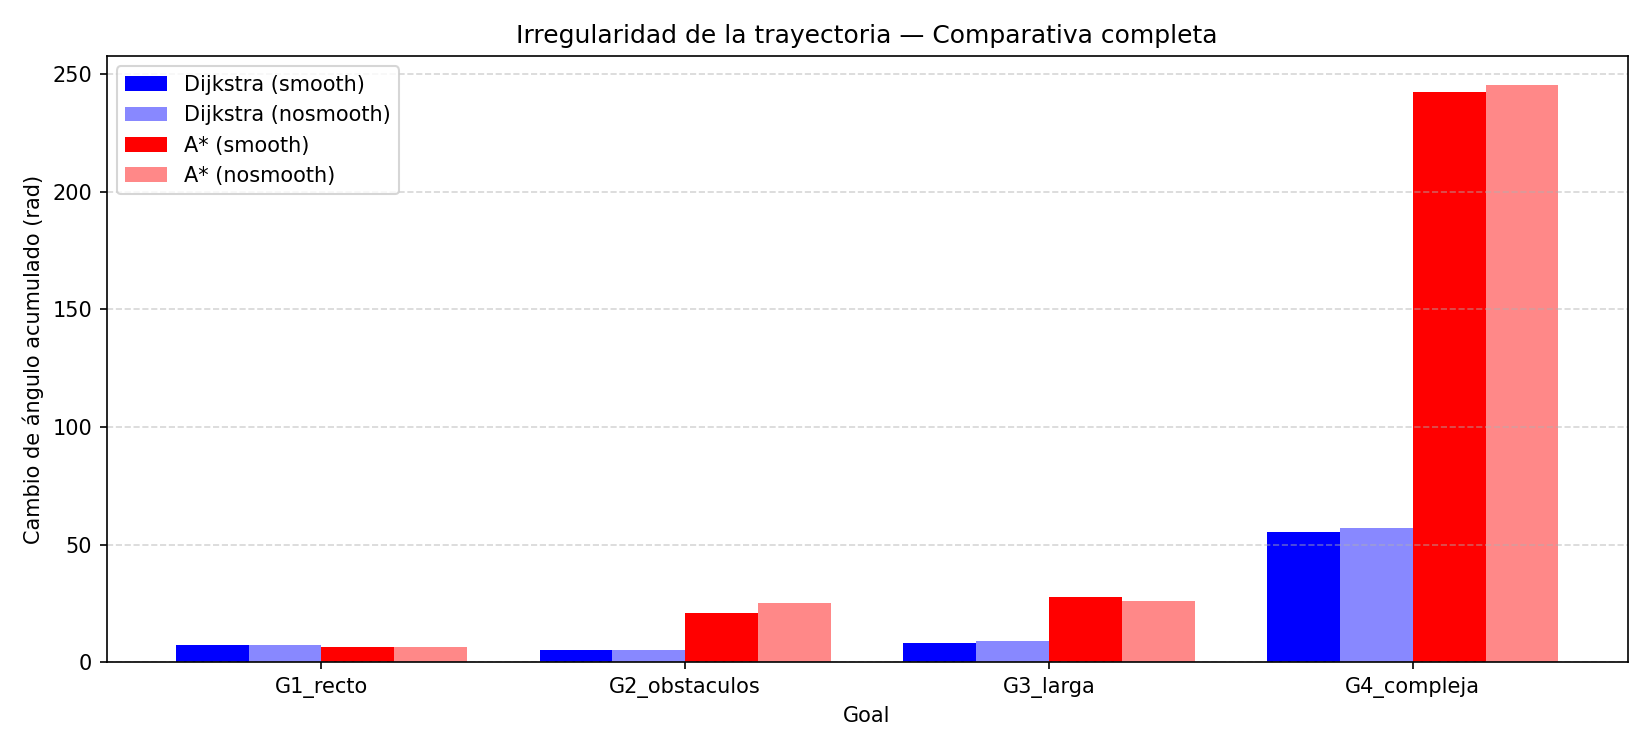
\includegraphics[width=0.85\textwidth]{figures/plots/static/4_smoothness_all}
    \caption{Irregularidad de la trayectoria — Comparativa completa de las cuatro configuraciones.}
    \label{fig:smoothness_all}
\end{figure}

El hallazgo más relevante del análisis estático es la diferencia radical en irregularidad entre Dijkstra y A*. En el objetivo más exigente (\texttt{goal4\_compleja}), Dijkstra smooth produce una irregularidad de 55,2 rad y Dijkstra nosmooth de 57,1 rad. A* smooth alcanza los 242,2 rad y A* nosmooth los 245,4 rad, lo que supone una irregularidad aproximadamente 4,4 veces mayor que la de Dijkstra.

En los objetivos más sencillos (\texttt{goal1\_recto} y \texttt{goal3\_larga}) las diferencias son pequeñas en todos los algoritmos: con pocos obstáculos que rodear, ambos algoritmos producen planes geométricamente similares. La divergencia aparece con fuerza en \texttt{goal2\_obstaculos} (Dijkstra: 5,2 rad, A*: 21--25 rad) y se amplifica en \texttt{goal4\_compleja}, donde la mayor densidad de obstáculos obliga a A* a generar trayectorias con cambios de dirección muy frecuentes.

La figura~\ref{fig:serrado_astar} ilustra visualmente este comportamiento: la trayectoria planificada por A* nosmooth presenta un patrón en zigzag característico de los algoritmos de búsqueda en cuadrícula cuando la heurística prioriza avanzar hacia el destino a través de celdas diagonales. Este patrón no aparece en las trayectorias de Dijkstra, que expande de forma uniforme y genera caminos más regulares.

\begin{figure}[H]
    \centering
    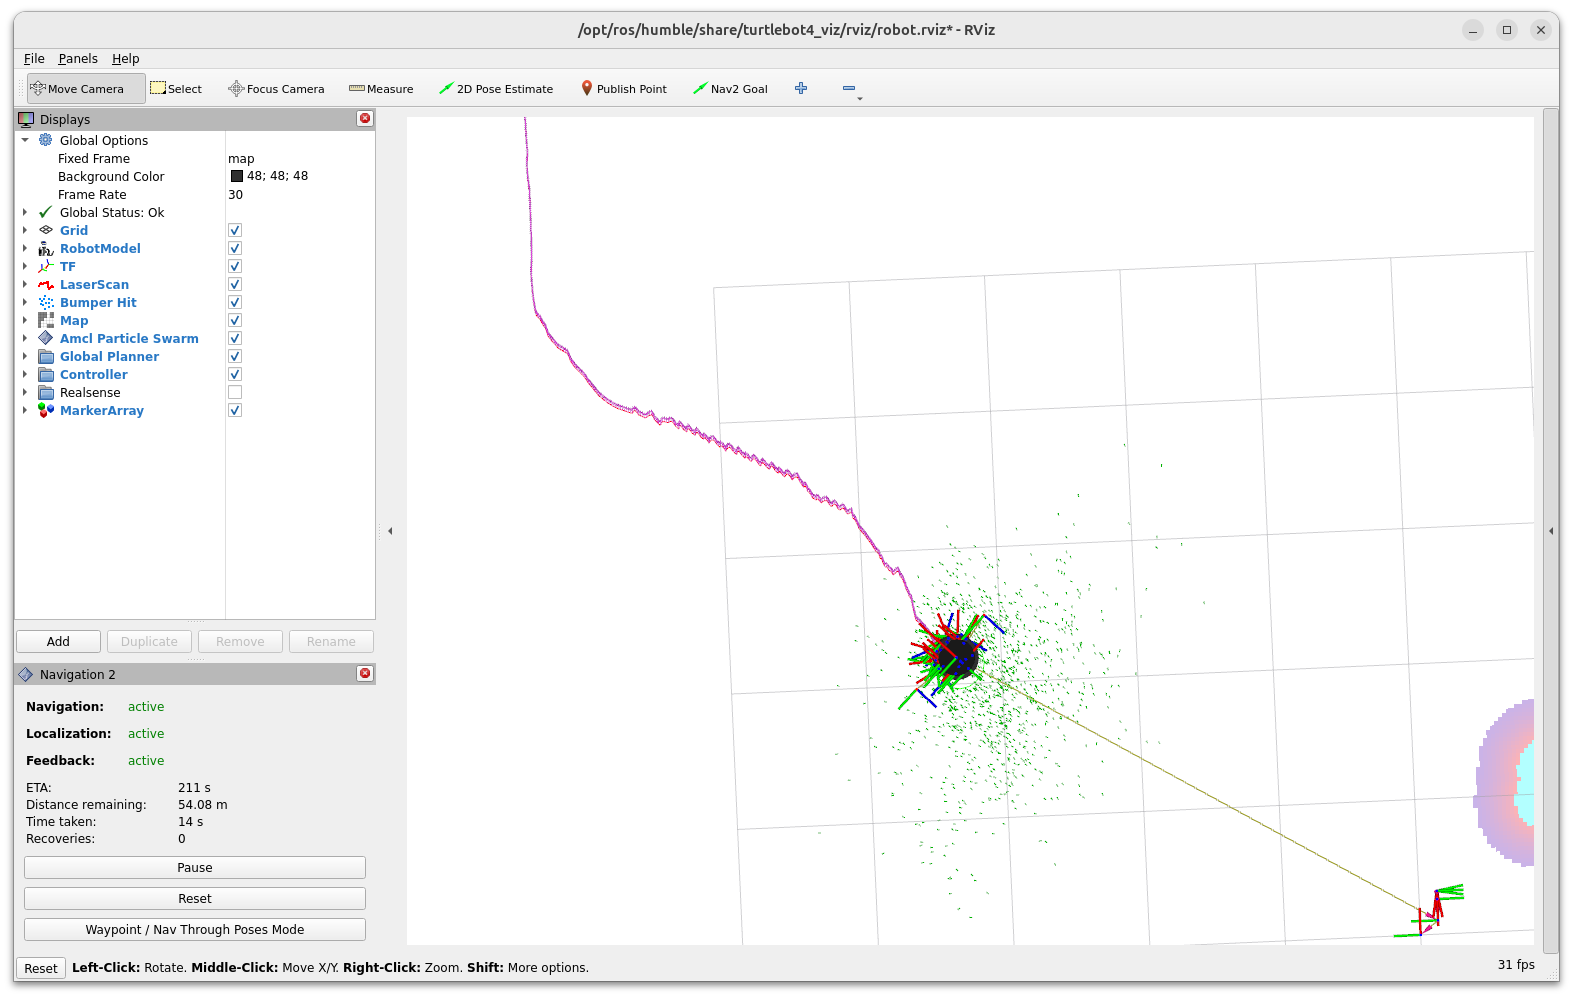
\includegraphics[width=0.65\textwidth]{figures/screenshots/serrado-en-trayectoria_astar-nosmooth}
    \caption{Patrón en zigzag de la trayectoria planificada por A* nosmooth, visible en RViz2 durante la navegación.}
    \label{fig:serrado_astar}
\end{figure}

Respecto al efecto del suavizado, su impacto sobre la irregularidad es mínimo en ambos algoritmos. En Dijkstra la diferencia entre smooth y nosmooth es inferior a 2 rad en todos los objetivos; en A*, inferior a 4 rad. El suavizado de NavFn reduce ligeramente la irregularidad pero no corrige el patrón estructural del algoritmo.

\subsection{Curvatura media}

Las figuras~\ref{fig:curvature_smooth}, \ref{fig:curvature_nosmooth} y \ref{fig:curvature_all} muestran la curvatura media de la trayectoria en rad/m, que normaliza la irregularidad respecto a la longitud del plan y permite comparar objetivos de distinta extensión.

\begin{figure}[H]
    \centering
    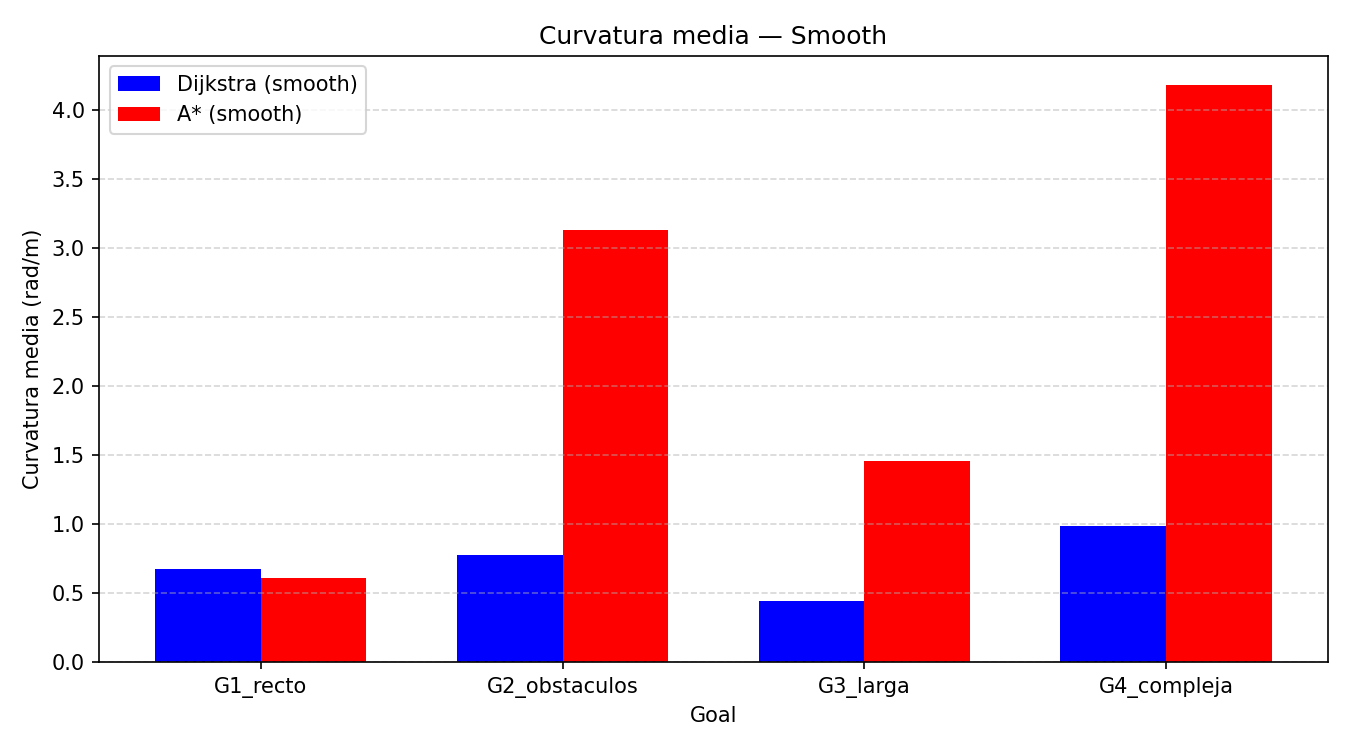
\includegraphics[width=0.85\textwidth]{figures/plots/static/5_curvature_smooth}
    \caption{Curvatura media — Dijkstra smooth vs A* smooth.}
    \label{fig:curvature_smooth}
\end{figure}

\begin{figure}[H]
    \centering
    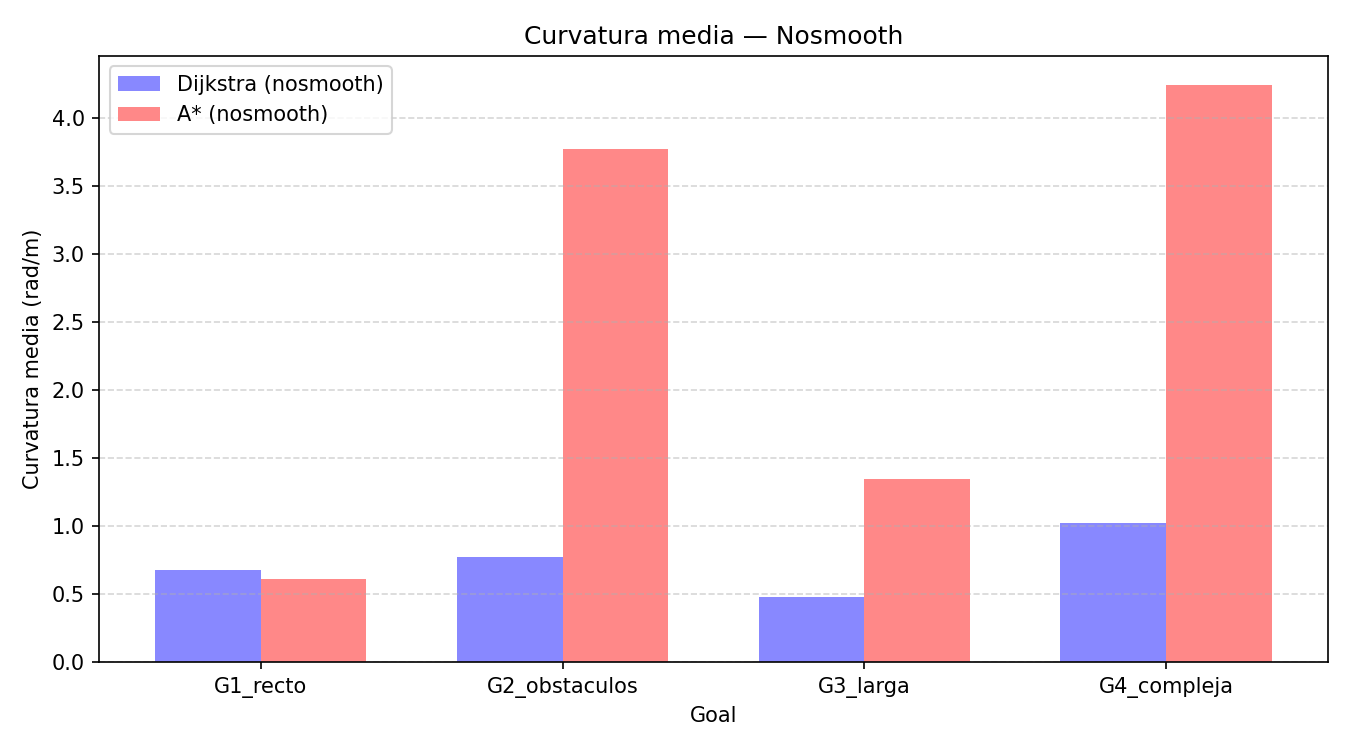
\includegraphics[width=0.85\textwidth]{figures/plots/static/6_curvature_nosmooth}
    \caption{Curvatura media — Dijkstra nosmooth vs A* nosmooth.}
    \label{fig:curvature_nosmooth}
\end{figure}

\begin{figure}[H]
    \centering
    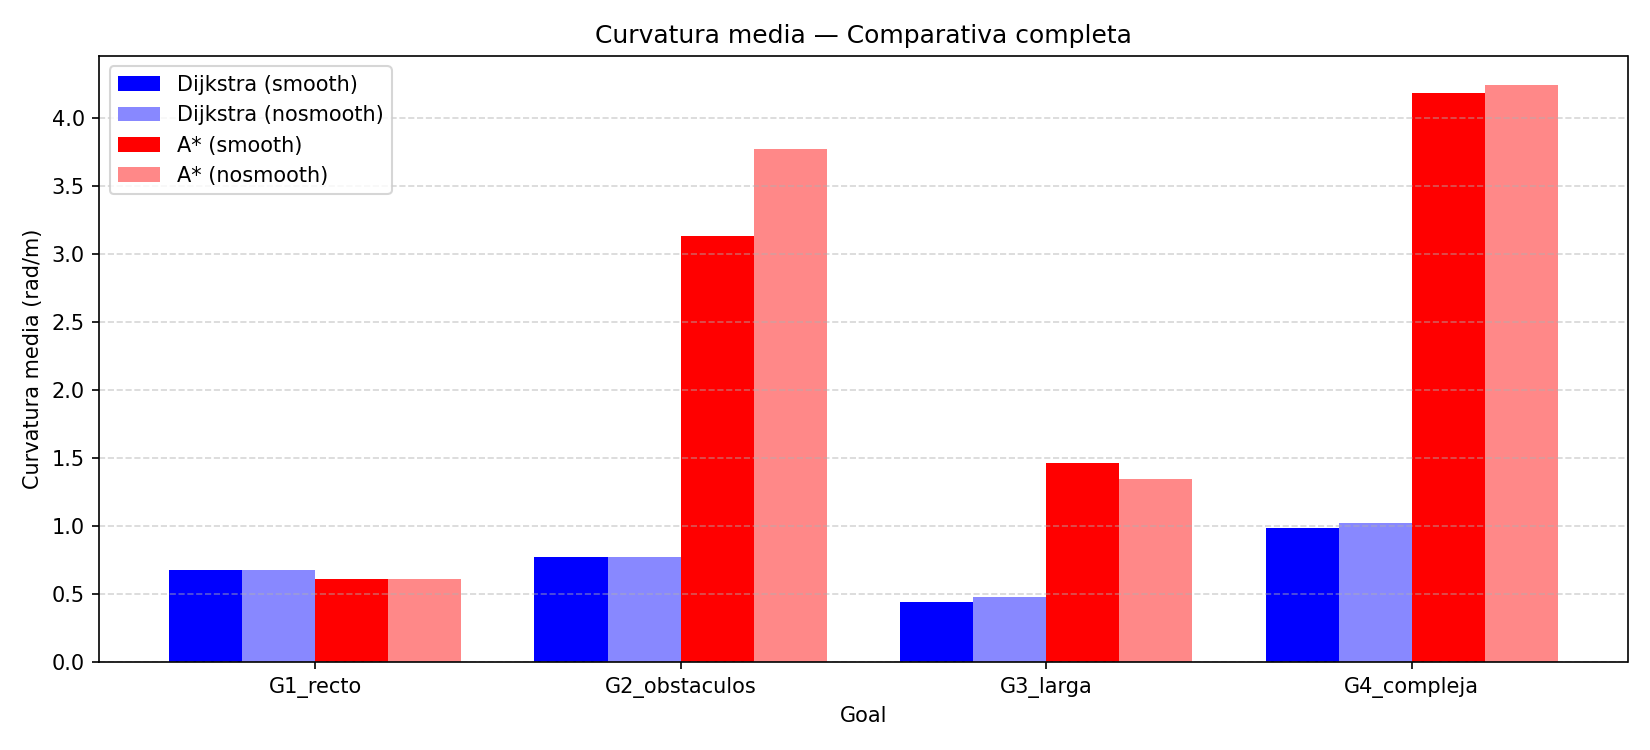
\includegraphics[width=0.85\textwidth]{figures/plots/static/7_curvature_all}
    \caption{Curvatura media — Comparativa completa de las cuatro configuraciones.}
    \label{fig:curvature_all}
\end{figure}

Los resultados confirman y matizan lo observado en los resultados de irregularidad. En \texttt{goal1\_recto}, todos los algoritmos producen curvaturas similares (0,61--0,68 rad/m), ya que la trayectoria es prácticamente directa. En \texttt{goal2\_obstaculos}, Dijkstra se mantiene en torno a 0,77 rad/m mientras que A* smooth alcanza 3,13 rad/m y A* nosmooth 3,77 rad/m. En \texttt{goal4\_compleja}, Dijkstra produce una curvatura media de ~1,0 rad/m frente a los ~4,2 rad/m de A*. La diferencia es consistente: A* genera trayectorias con una densidad de giros entre 3 y 5 veces mayor que Dijkstra en los objetivos con obstáculos.

En cuanto al efecto del suavizado sobre la curvatura media, el comportamiento es mayoritariamente favorable: smooth produce menor curvatura que nosmooth en casi todos los objetivos, aunque la reducción es modesta (inferior al 20\% en la mayoría de los casos). La excepción es \texttt{goal3\_larga}, donde A* nosmooth presenta una curvatura ligeramente menor que A* smooth (1,35 vs 1,46 rad/m), sin una causa clara más allá de la particularidad geométrica de esa trayectoria.

\section{Resultados dinámicos}

Las métricas dinámicas se obtienen durante la ejecución real del robot navegando hasta \texttt{goal4\_compleja} $(-13, 19)$, el objetivo más complejo del entorno. El robot recorre una trayectoria de aproximadamente 58 metros en un entorno con múltiples obstáculos y cambios de dirección.

\begin{tcolorbox}[colback=gray!10, colframe=gray!40, title=Vídeo de la navegación]
Se ha grabado un vídeo de la navegación completa del robot simulado hasta \texttt{goal4\_compleja} con la configuración Dijkstra smooth, que incluye la visualización en RViz2 del costmap, las partículas AMCL y la trayectoria ejecutada en tiempo real. El vídeo está disponible en:\\
\url{https://youtu.be/K-22qo7MT1w}
\end{tcolorbox}

\subsection{Trayectorias ejecutadas}

Las figuras~\ref{fig:par_dijkstra}--\ref{fig:par_astar_nosmooth} muestran, para cada configuración, la trayectoria planificada tal como se visualiza en RViz2 junto con su reconstrucción a partir del CSV de métricas.

\begin{figure}[H]
    \centering
    \begin{minipage}{0.48\textwidth}
        \centering
        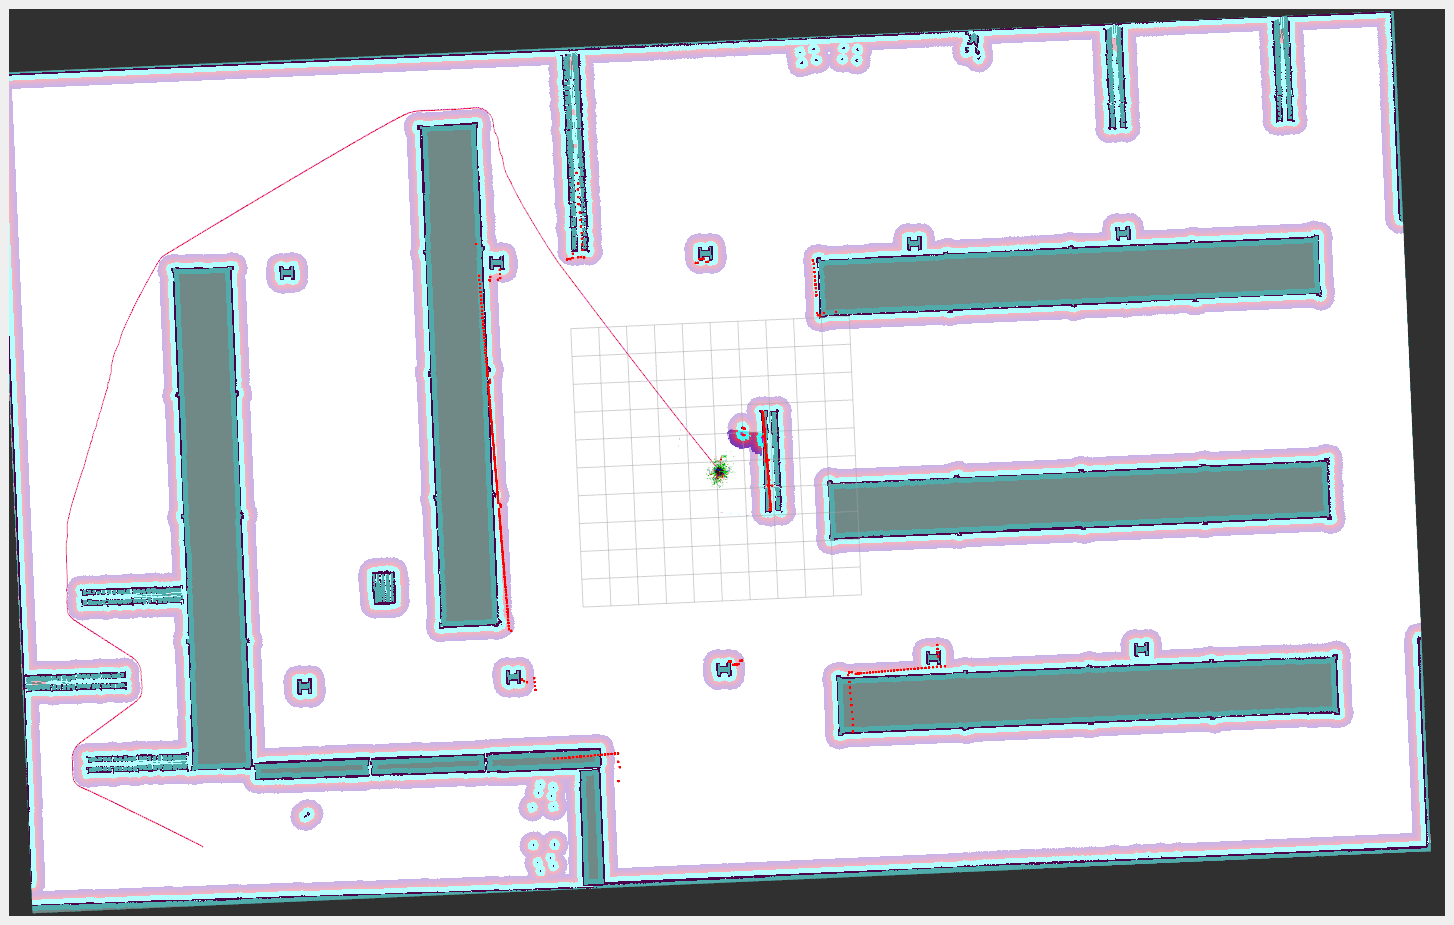
\includegraphics[width=\textwidth]{figures/screenshots/screenshot_final_dijkstra}
    \end{minipage}
    \hfill
    \begin{minipage}{0.48\textwidth}
        \centering
        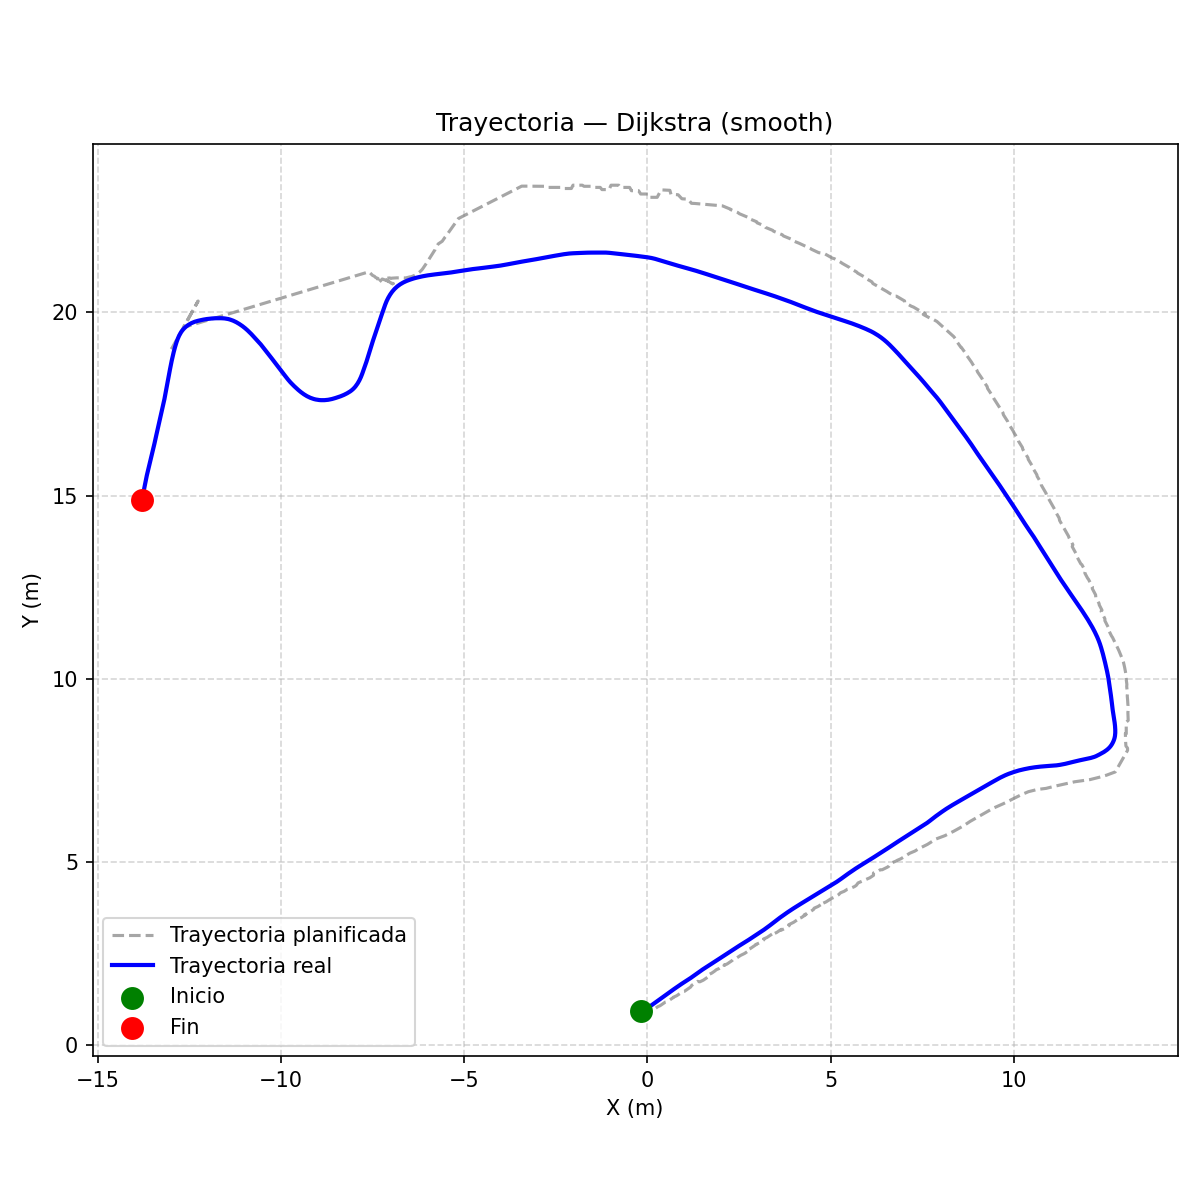
\includegraphics[width=\textwidth]{figures/plots/dynamic/1_trajectory_dijkstra}
    \end{minipage}
    \caption{Trayectoria Dijkstra smooth: vista en RViz2 (izquierda) y reconstrucción desde CSV (derecha).}
    \label{fig:par_dijkstra}
\end{figure}

\begin{figure}[H]
    \centering
    \begin{minipage}{0.48\textwidth}
        \centering
        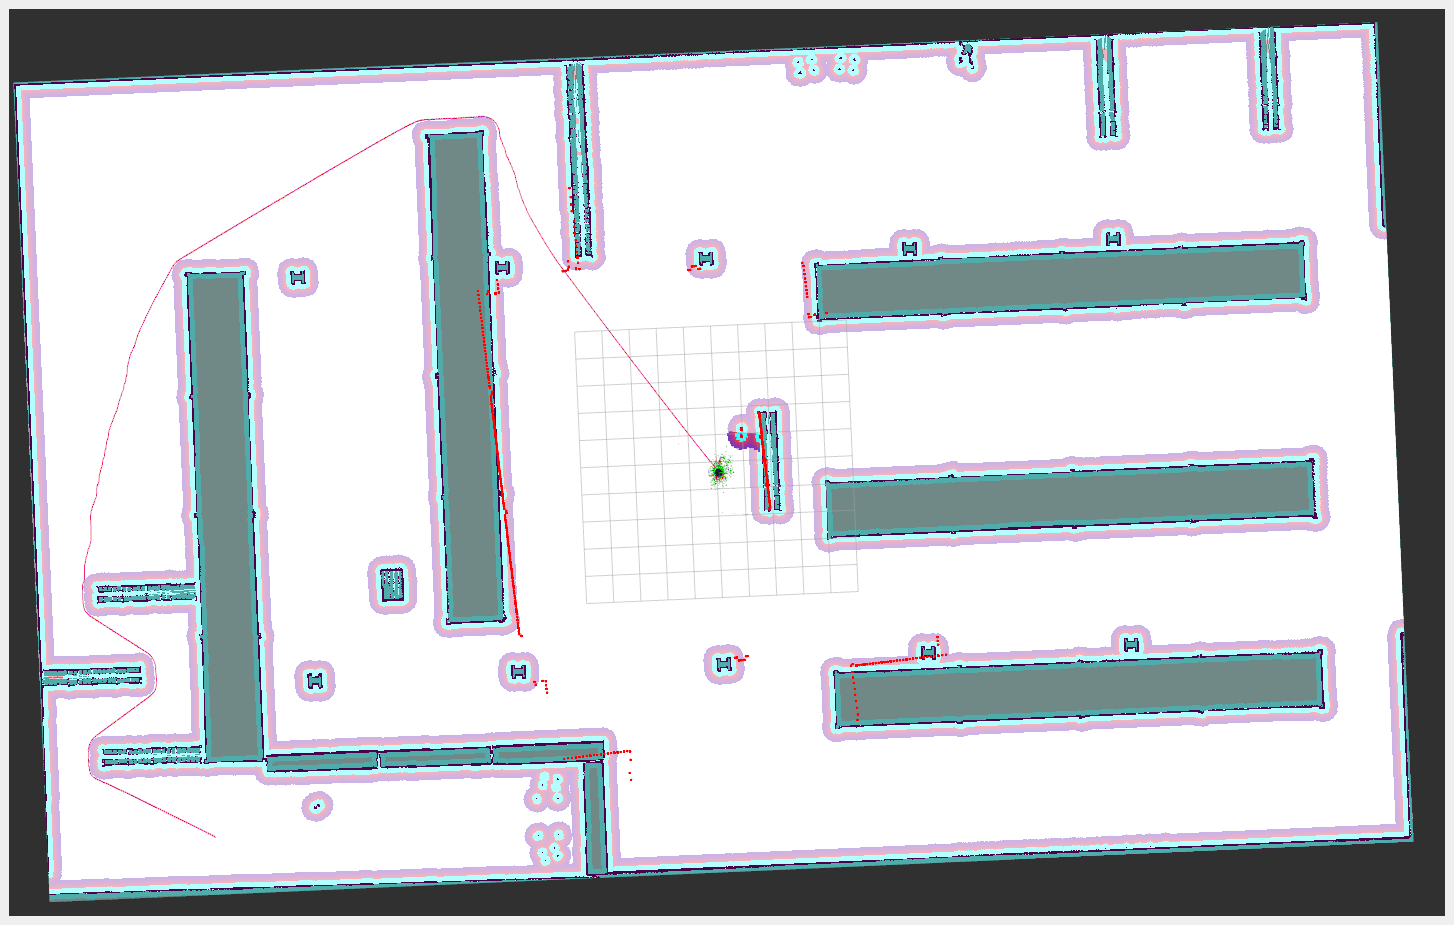
\includegraphics[width=\textwidth]{figures/screenshots/screenshot_final_dijkstra_nosmooth}
    \end{minipage}
    \hfill
    \begin{minipage}{0.48\textwidth}
        \centering
        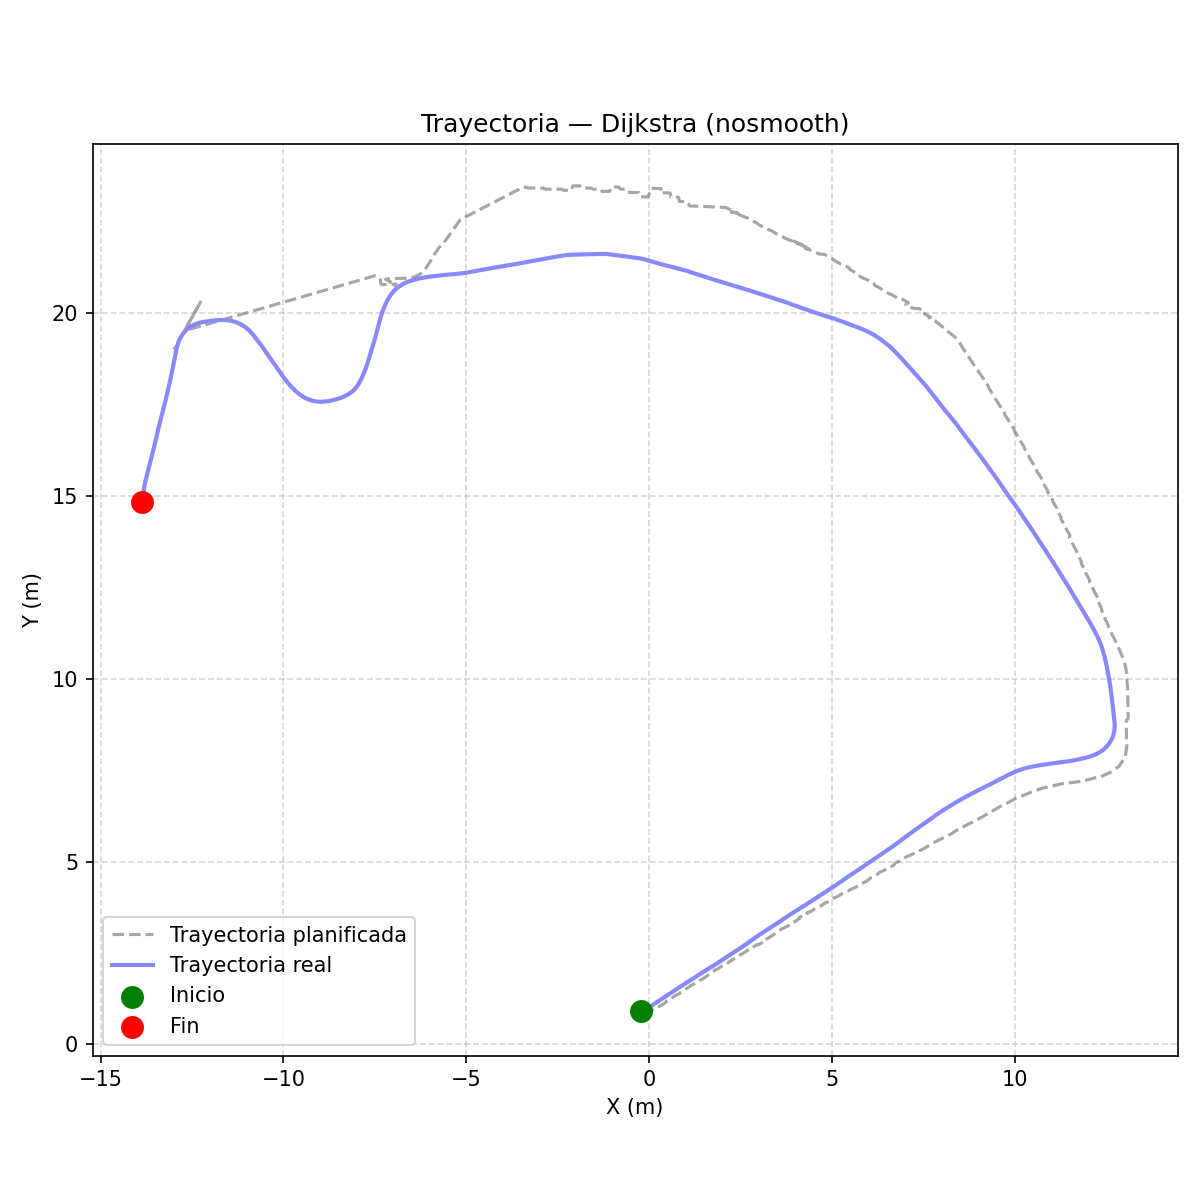
\includegraphics[width=\textwidth]{figures/plots/dynamic/2_trajectory_dijkstra_nosmooth}
    \end{minipage}
    \caption{Trayectoria Dijkstra nosmooth: vista en RViz2 (izquierda) y reconstrucción desde CSV (derecha).}
    \label{fig:par_dijkstra_nosmooth}
\end{figure}

\begin{figure}[H]
    \centering
    \begin{minipage}{0.48\textwidth}
        \centering
        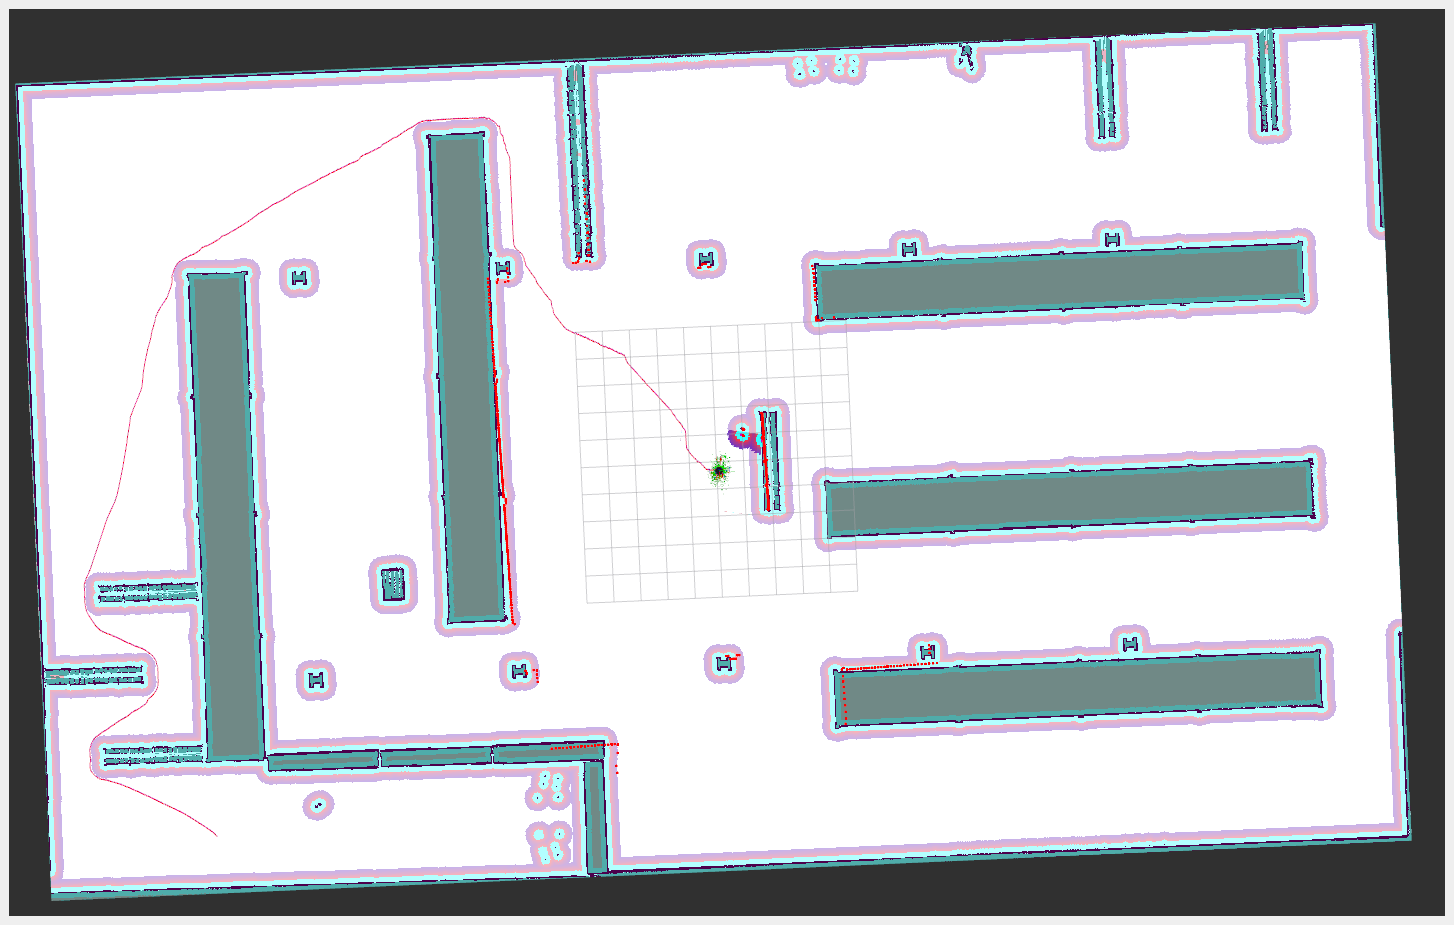
\includegraphics[width=\textwidth]{figures/screenshots/screenshot_final_astar}
    \end{minipage}
    \hfill
    \begin{minipage}{0.48\textwidth}
        \centering
        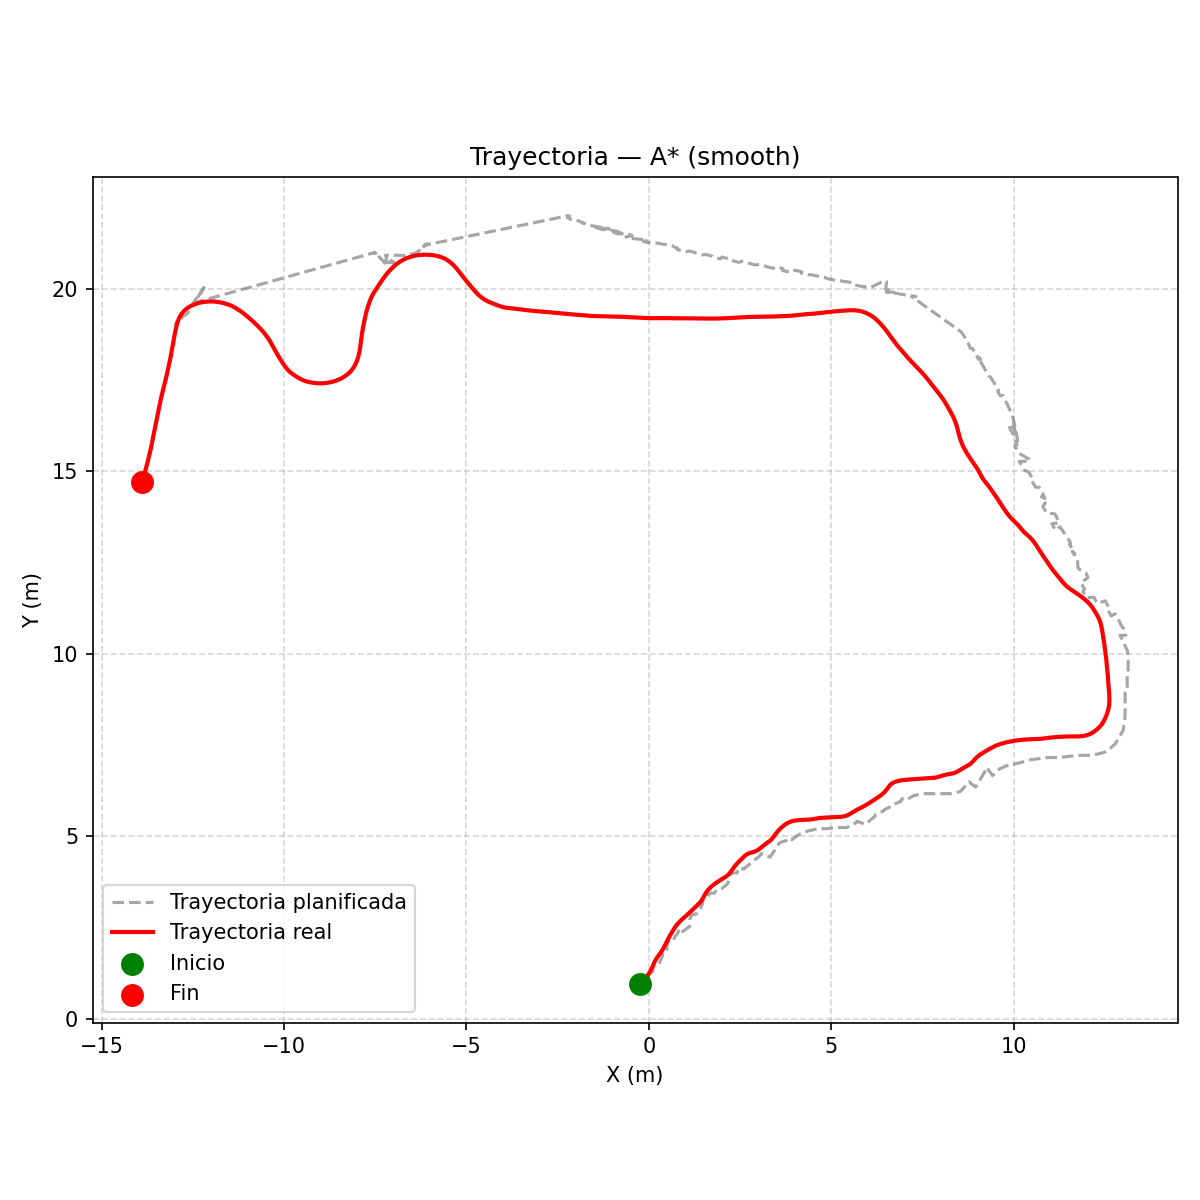
\includegraphics[width=\textwidth]{figures/plots/dynamic/3_trajectory_astar}
    \end{minipage}
    \caption{Trayectoria A* smooth: vista en RViz2 (izquierda) y reconstrucción desde CSV (derecha).}
    \label{fig:par_astar}
\end{figure}

\begin{figure}[H]
    \centering
    \begin{minipage}{0.48\textwidth}
        \centering
        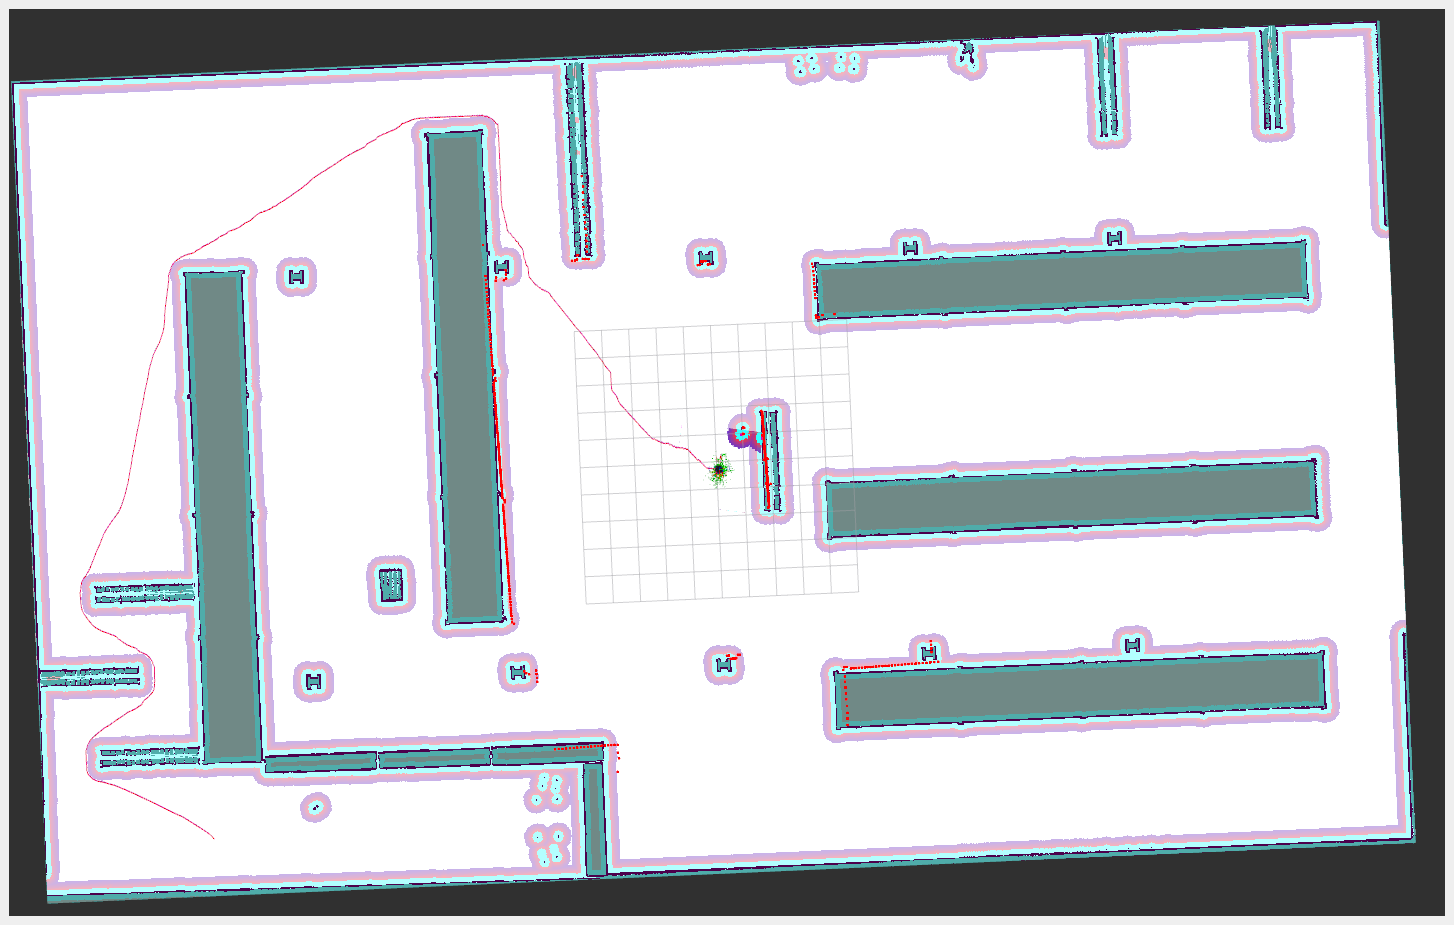
\includegraphics[width=\textwidth]{figures/screenshots/screenshot_final_astar_nosmooth}
    \end{minipage}
    \hfill
    \begin{minipage}{0.48\textwidth}
        \centering
        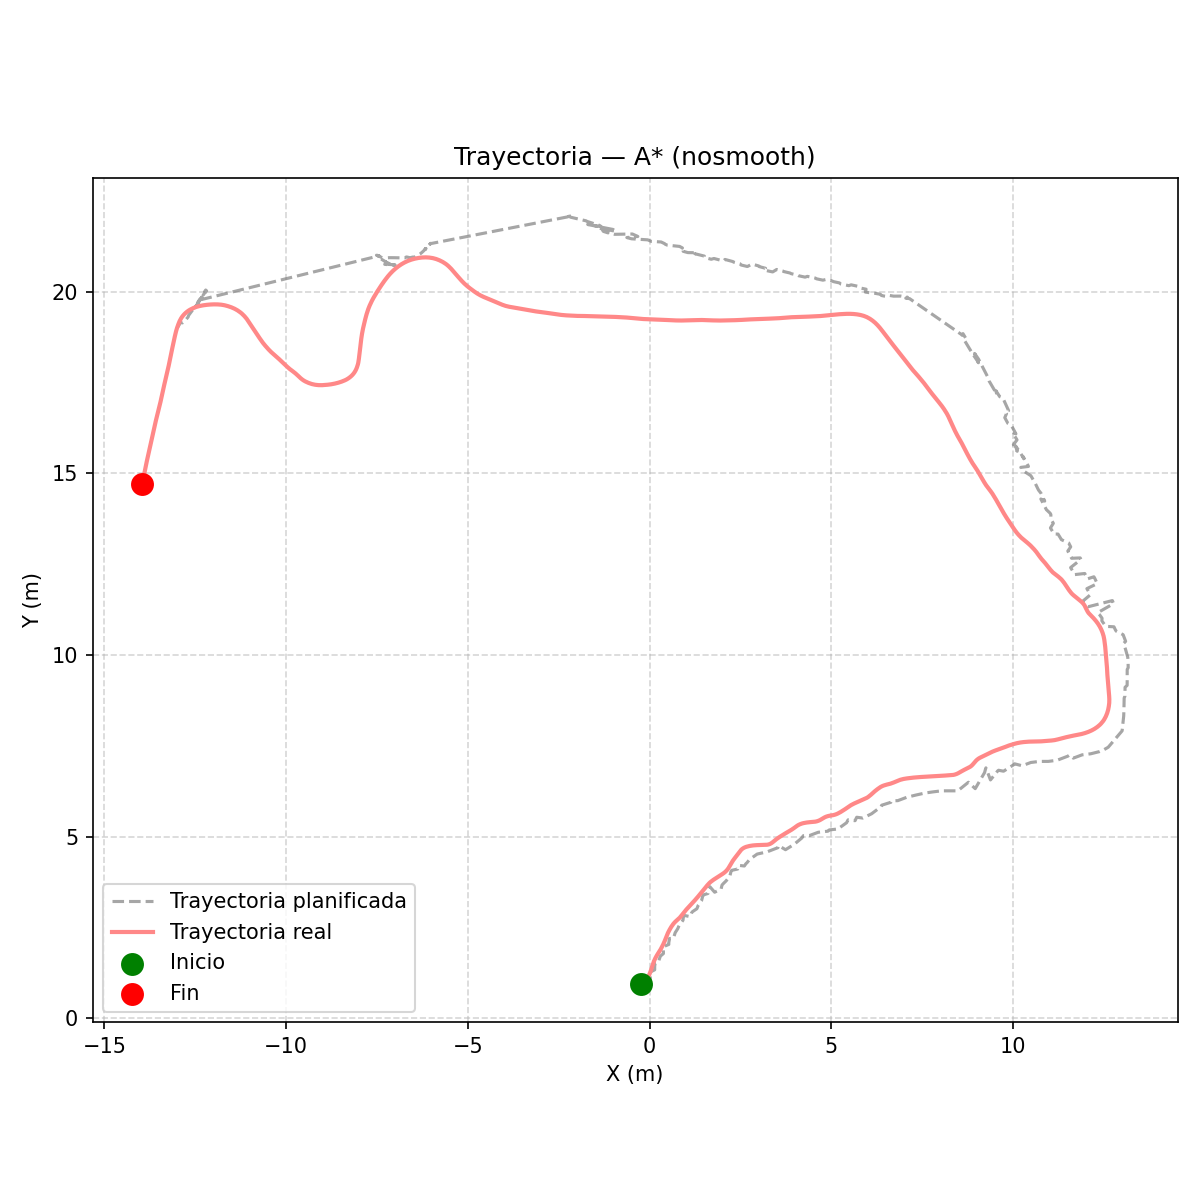
\includegraphics[width=\textwidth]{figures/plots/dynamic/4_trajectory_astar_nosmooth}
    \end{minipage}
    \caption{Trayectoria A* nosmooth: vista en RViz2 (izquierda) y reconstrucción desde CSV (derecha).}
    \label{fig:par_astar_nosmooth}
\end{figure}

Las cuatro trayectorias reales son prácticamente idénticas en forma, lo que indica que el controlador local DWB produce un comportamiento de navegación similar independientemente del planificador global utilizado. Comparando la vista de RViz2 con la reconstrucción desde CSV, se aprecia que la trayectoria planificada reconstruida presenta discontinuidades en la zona inferior derecha del mapa, debidas a replanificaciones de Nav2 durante la navegación tal y como se describe en el capítulo de metodología (\ref{sec:limitaciones_simulacion}). La trayectoria planificada real sí rodea correctamente todos los obstáculos, como confirma la vista de RViz2.

\subsection{Velocidades de navegación}

Las figuras~\ref{fig:vel_dijkstra}--\ref{fig:vel_astar_nosmooth} muestran la evolución de la velocidad lineal y angular durante la navegación para cada configuración.

\begin{figure}[H]
    \centering
    \begin{minipage}{0.48\textwidth}
        \centering
        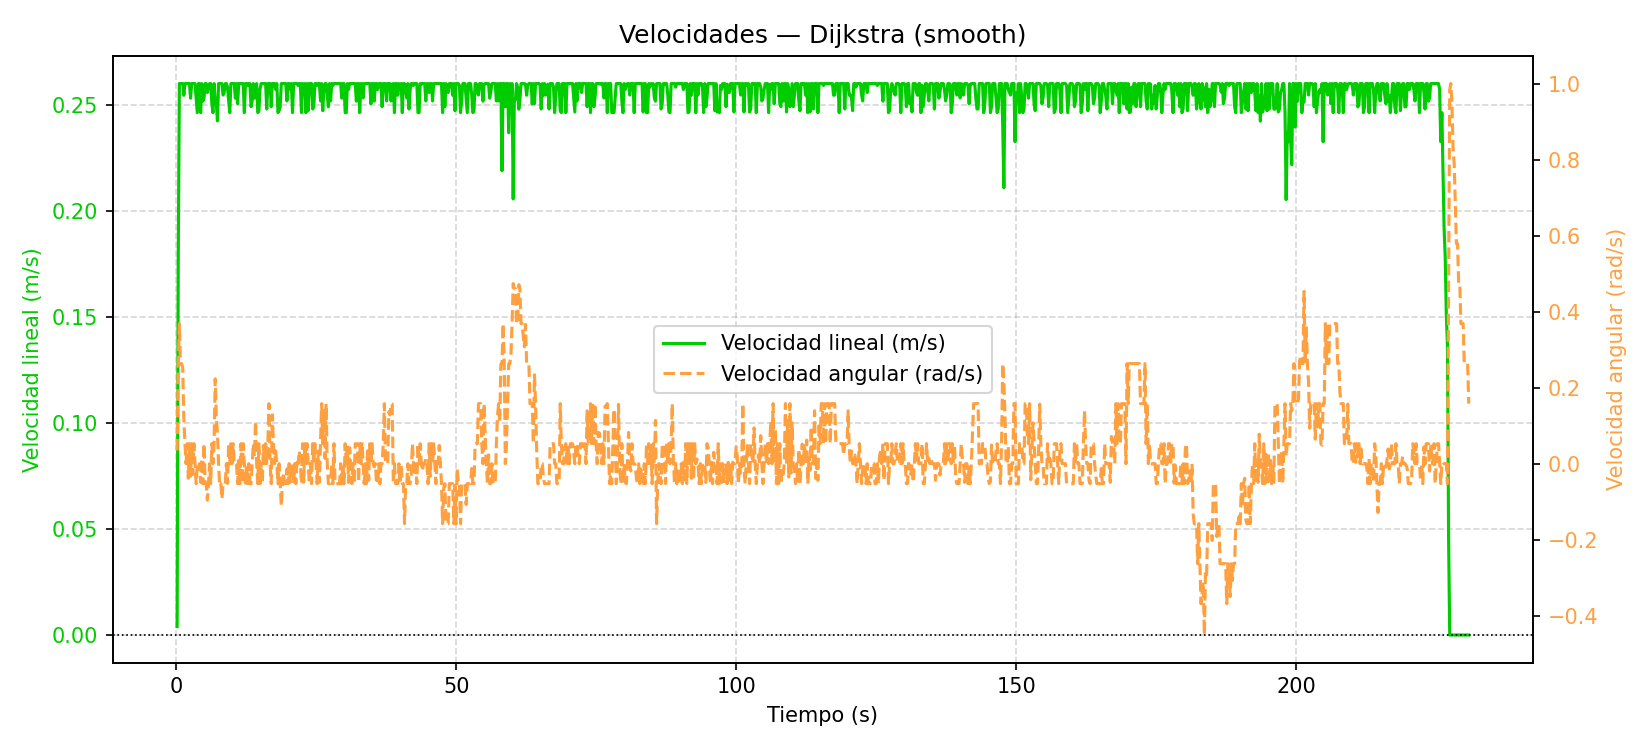
\includegraphics[width=\textwidth]{figures/plots/dynamic/5_velocities_dijkstra}
        \caption{Velocidades — Dijkstra smooth.}
        \label{fig:vel_dijkstra}
    \end{minipage}
    \hfill
    \begin{minipage}{0.48\textwidth}
        \centering
        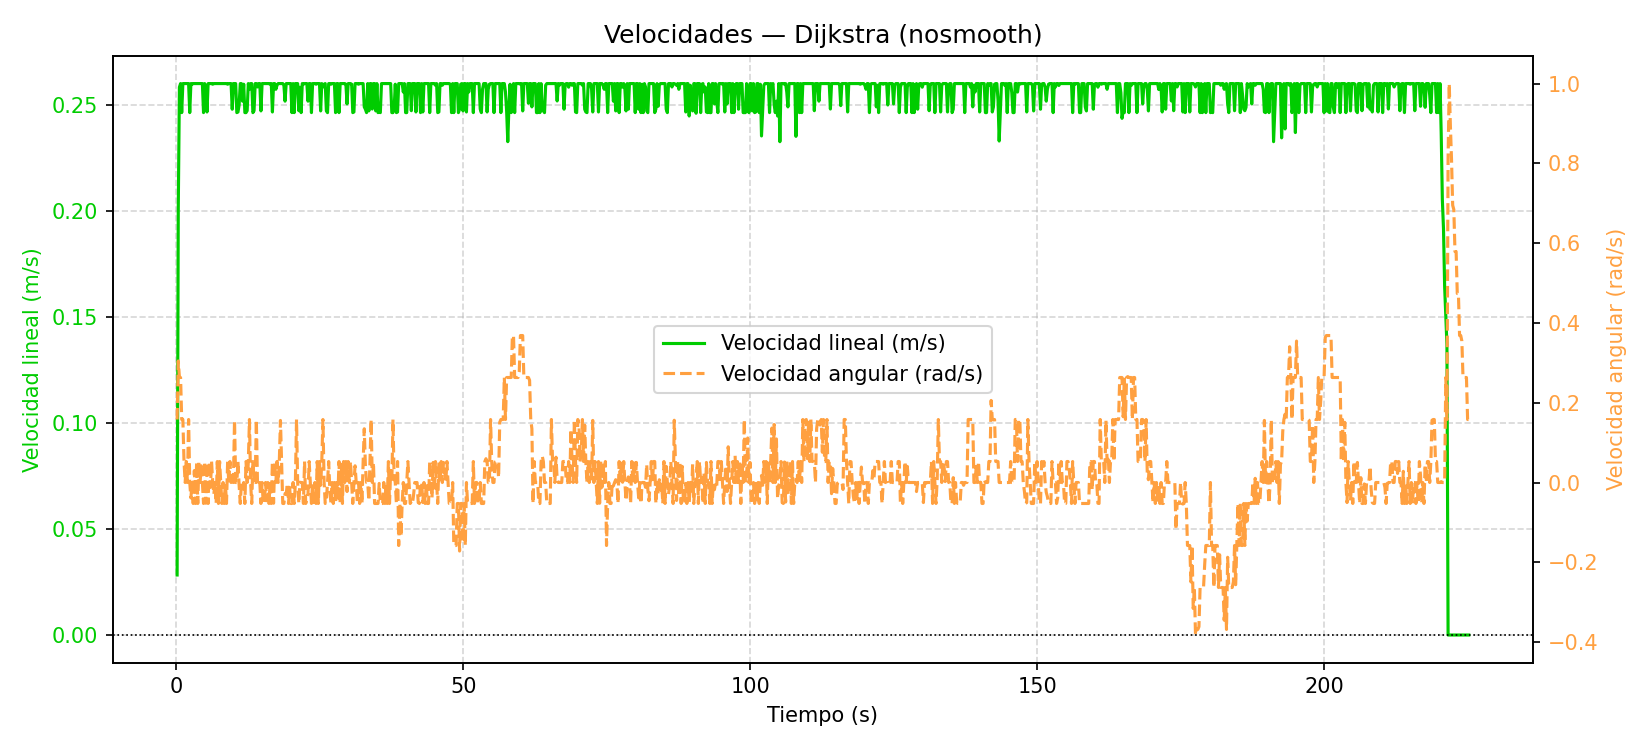
\includegraphics[width=\textwidth]{figures/plots/dynamic/6_velocities_dijkstra_nosmooth}
        \caption{Velocidades — Dijkstra nosmooth.}
        \label{fig:vel_dijkstra_nosmooth}
    \end{minipage}
\end{figure}

\begin{figure}[H]
    \centering
    \begin{minipage}{0.48\textwidth}
        \centering
        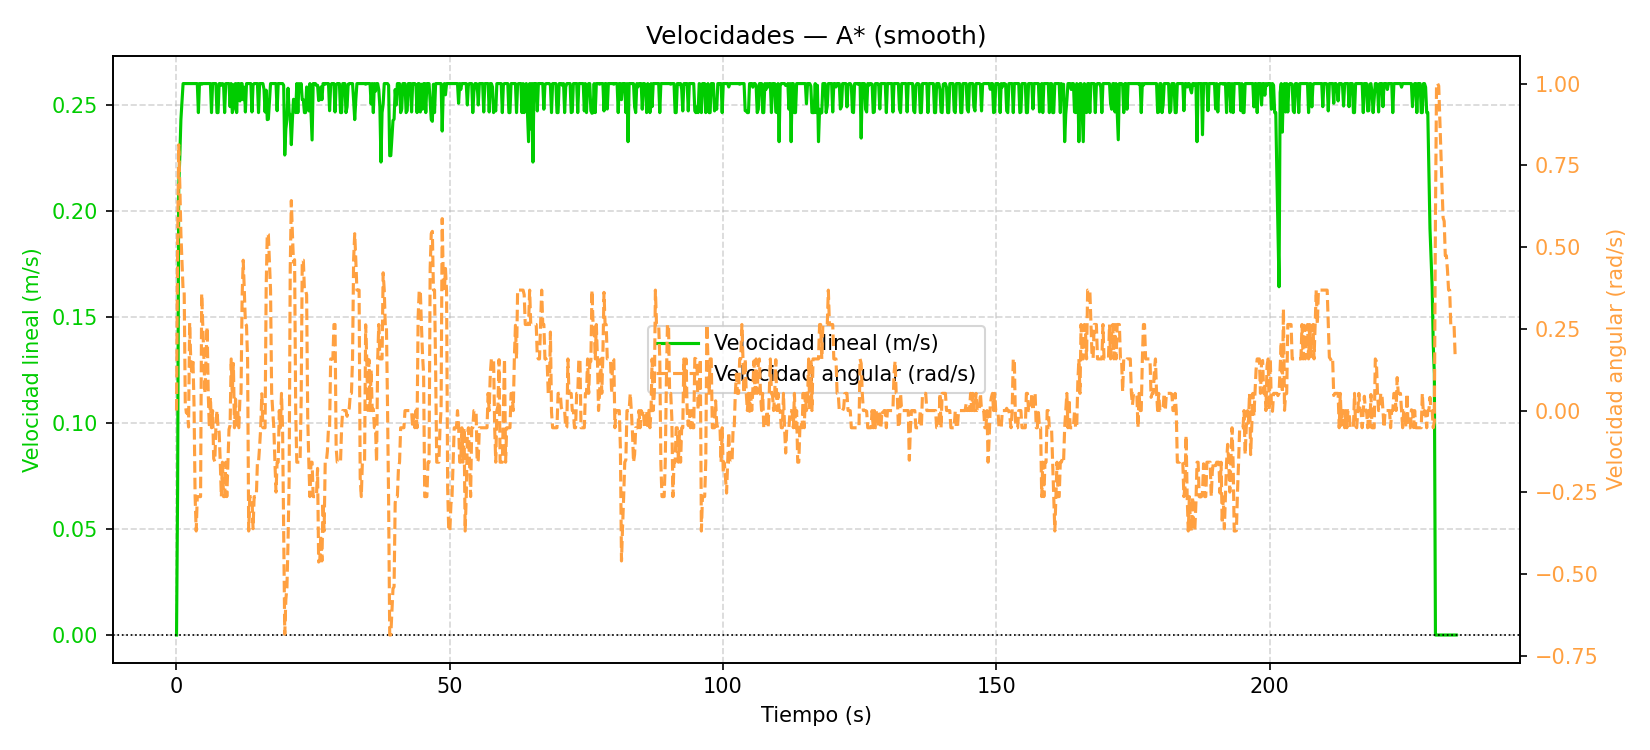
\includegraphics[width=\textwidth]{figures/plots/dynamic/7_velocities_astar}
        \caption{Velocidades — A* smooth.}
        \label{fig:vel_astar}
    \end{minipage}
    \hfill
    \begin{minipage}{0.48\textwidth}
        \centering
        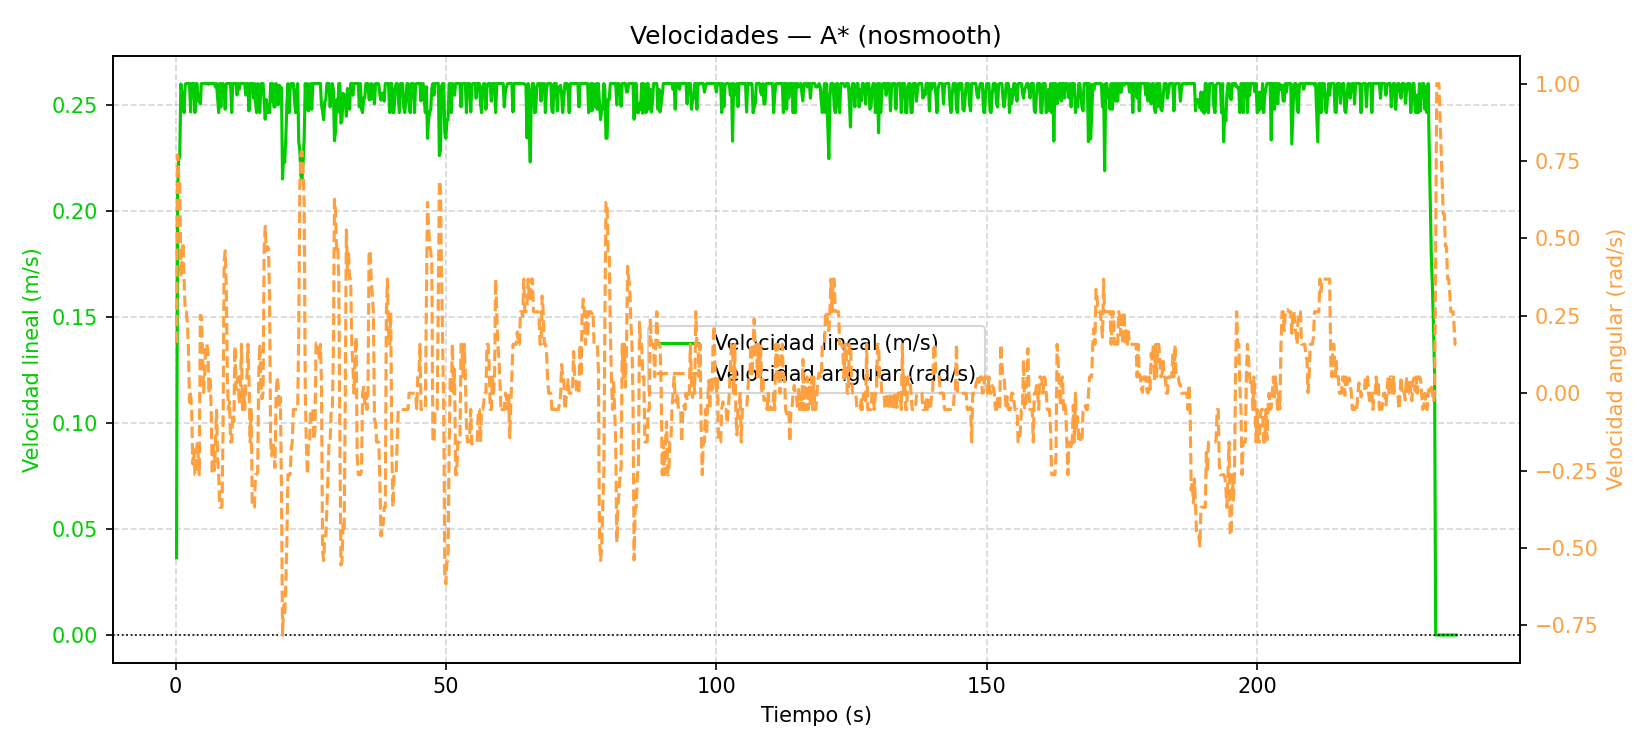
\includegraphics[width=\textwidth]{figures/plots/dynamic/8_velocities_astar_nosmooth}
        \caption{Velocidades — A* nosmooth.}
        \label{fig:vel_astar_nosmooth}
    \end{minipage}
\end{figure}

La velocidad lineal es prácticamente idéntica en las cuatro configuraciones: satura en 0,26 m/s durante la mayor parte del recorrido y cae puntualmente en los giros. La diferencia significativa está en la velocidad angular: en Dijkstra se mantiene en valores bajos y relativamente estables, con picos esporádicos de hasta ~0,16 rad/s. En A* smooth y A* nosmooth la velocidad angular es notablemente más errática, con oscilaciones frecuentes que alcanzan ~0,5 rad/s durante los primeros 50 segundos y a lo largo de todo el recorrido. Esto es la manifestación dinámica de las trayectorias más irregulares que genera A*: el controlador DWB debe realizar ajustes de dirección más frecuentes para seguir el plan.

\subsection{ETA calculado por Nav2}

Las figuras~\ref{fig:eta_dijkstra}--\ref{fig:eta_all} muestran la comparativa entre el tiempo restante real y el ETA calculado por Nav2, así como una comparativa de los cuatro algoritmos.

\begin{figure}[H]
    \centering
    \begin{minipage}{0.48\textwidth}
        \centering
        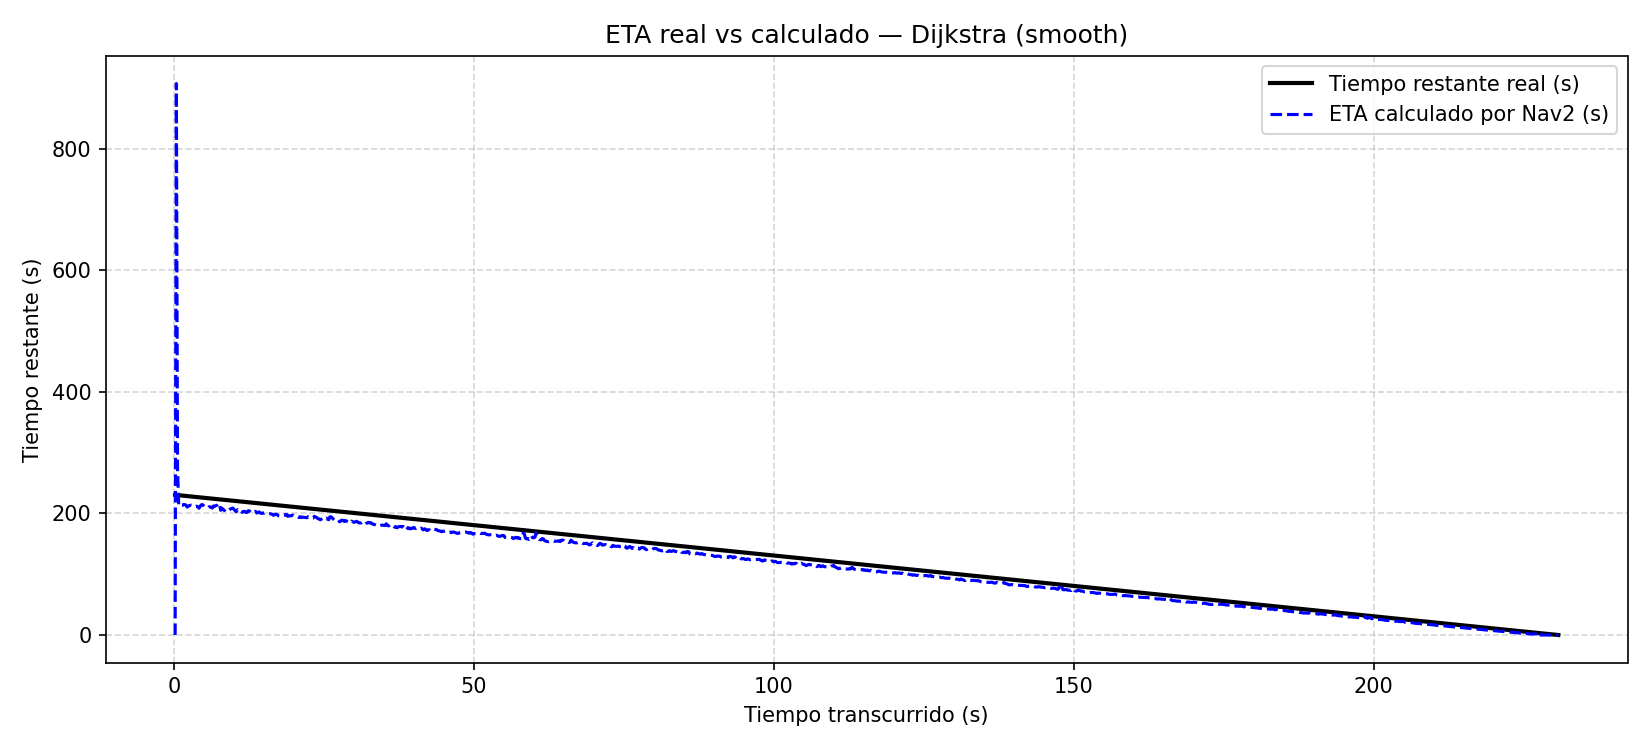
\includegraphics[width=\textwidth]{figures/plots/dynamic/9_eta_dijkstra}
        \caption{ETA real vs calculado — Dijkstra smooth.}
        \label{fig:eta_dijkstra}
    \end{minipage}
    \hfill
    \begin{minipage}{0.48\textwidth}
        \centering
        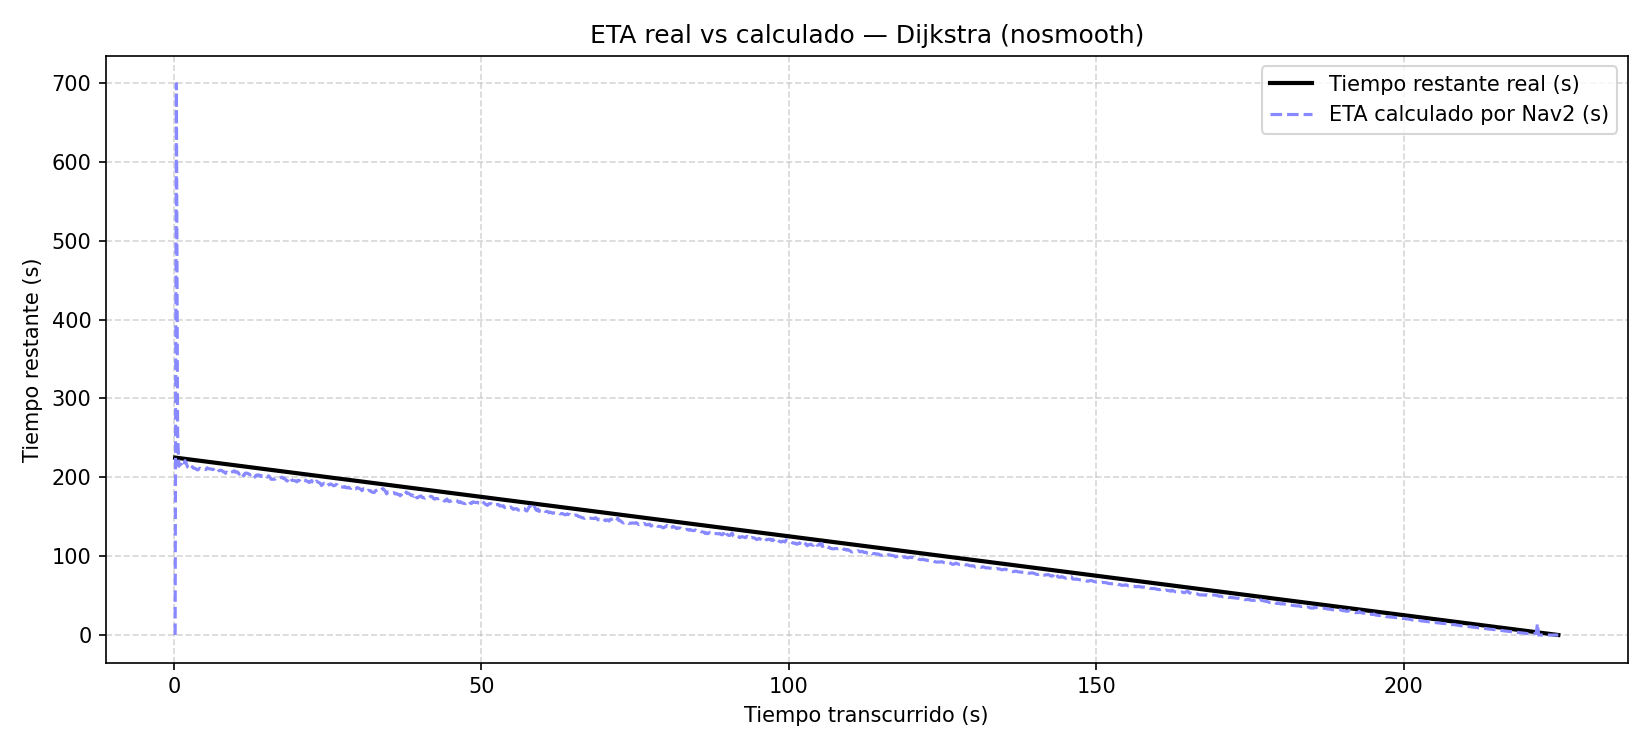
\includegraphics[width=\textwidth]{figures/plots/dynamic/10_eta_dijkstra_nosmooth}
        \caption{ETA real vs calculado — Dijkstra nosmooth.}
        \label{fig:eta_dijkstra_nosmooth}
    \end{minipage}
\end{figure}

\begin{figure}[H]
    \centering
    \begin{minipage}{0.48\textwidth}
        \centering
        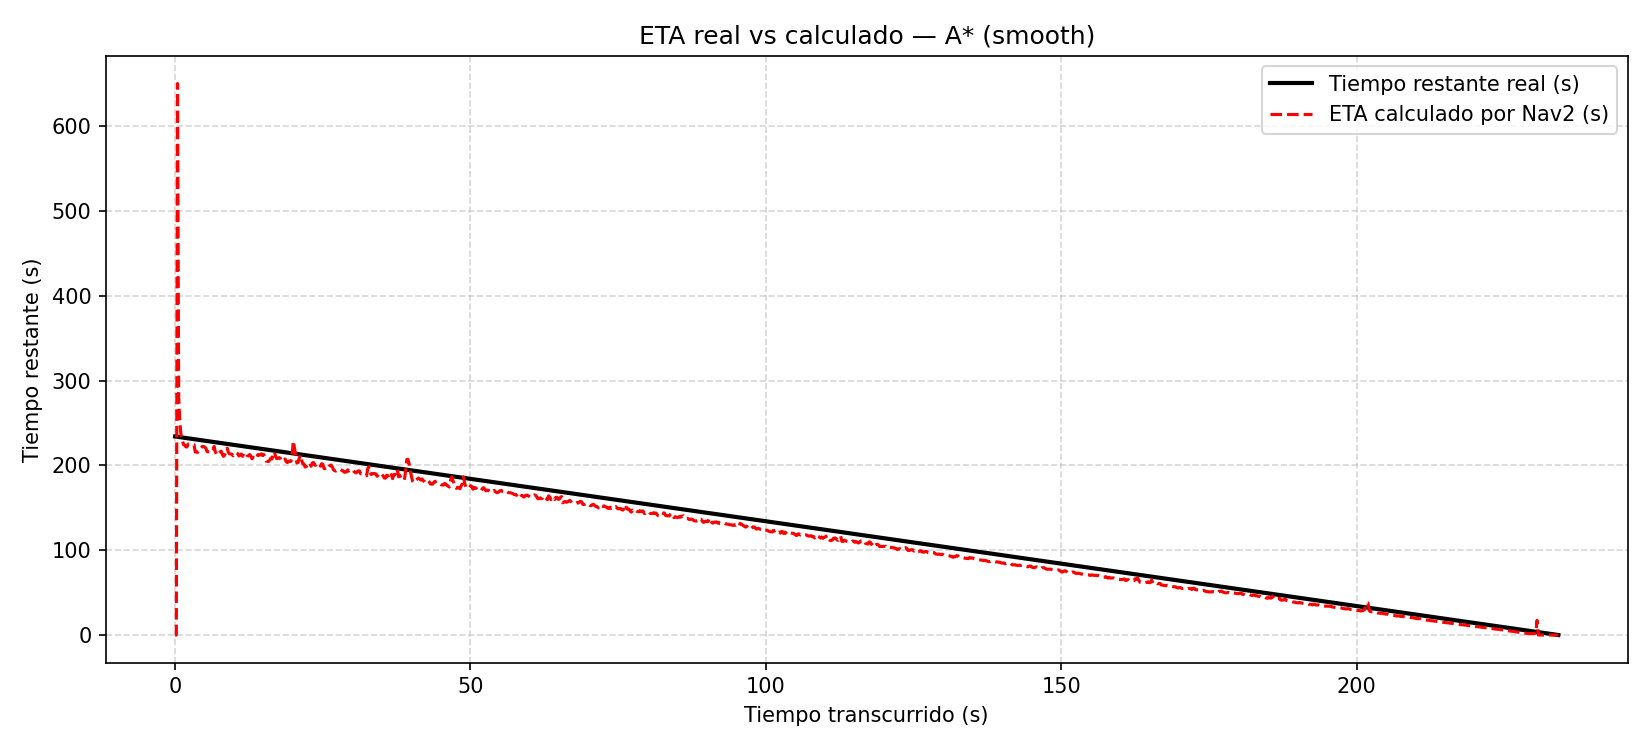
\includegraphics[width=\textwidth]{figures/plots/dynamic/11_eta_astar}
        \caption{ETA real vs calculado — A* smooth.}
        \label{fig:eta_astar}
    \end{minipage}
    \hfill
    \begin{minipage}{0.48\textwidth}
        \centering
        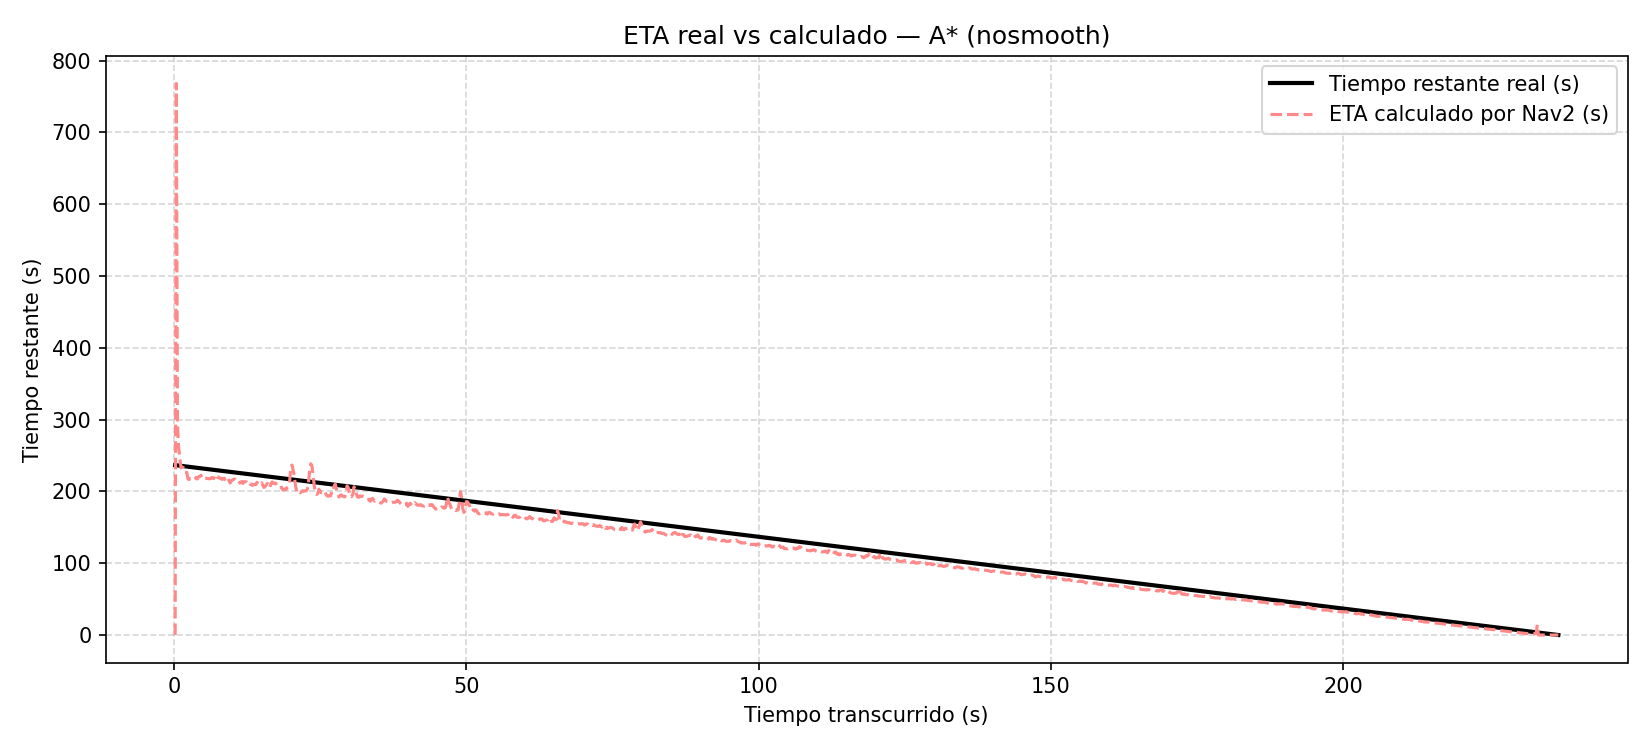
\includegraphics[width=\textwidth]{figures/plots/dynamic/12_eta_astar_nosmooth}
        \caption{ETA real vs calculado — A* nosmooth.}
        \label{fig:eta_astar_nosmooth}
    \end{minipage}
\end{figure}

\begin{figure}[H]
    \centering
    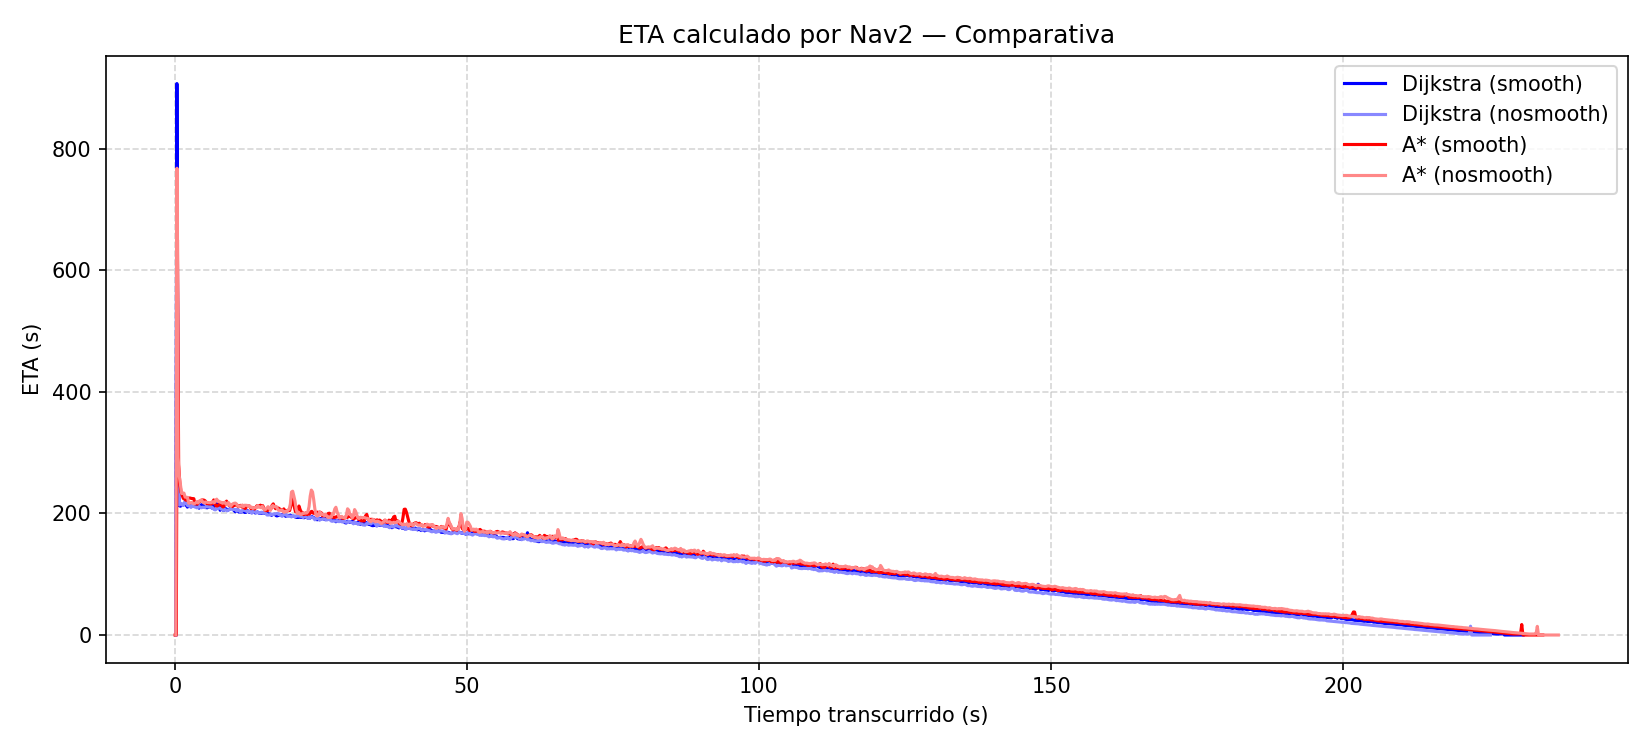
\includegraphics[width=0.9\textwidth]{figures/plots/dynamic/14_eta_all}
    \caption{ETA calculado por Nav2 — Comparativa de las cuatro configuraciones.}
    \label{fig:eta_all}
\end{figure}

En todos los casos, el primer valor de ETA registrado es anómalamente alto (entre 650 y 907 s), ya que el primer sample se toma antes de que Nav2 haya completado el cómputo del plan. Tras este pico inicial, el ETA cae bruscamente y se alinea con el tiempo restante real, siguiendo una evolución decreciente y aproximadamente lineal hasta el final de la navegación.

La diferencia más relevante entre algoritmos es visible en las curvas de A* (figuras~\ref{fig:eta_astar} y \ref{fig:eta_astar_nosmooth}): el ETA presenta escalones y saltos periódicos a lo largo de toda la navegación, que corresponden a replanificaciones de Nav2 provocadas por el alejamiento del robot respecto al plan. En Dijkstra, las curvas son más lisas e indican menos episodios de replanificación, lo que es coherente con la mayor suavidad de las trayectorias que genera este algoritmo.

\subsection{Tiempo total de navegación}

\begin{figure}[H]
    \centering
    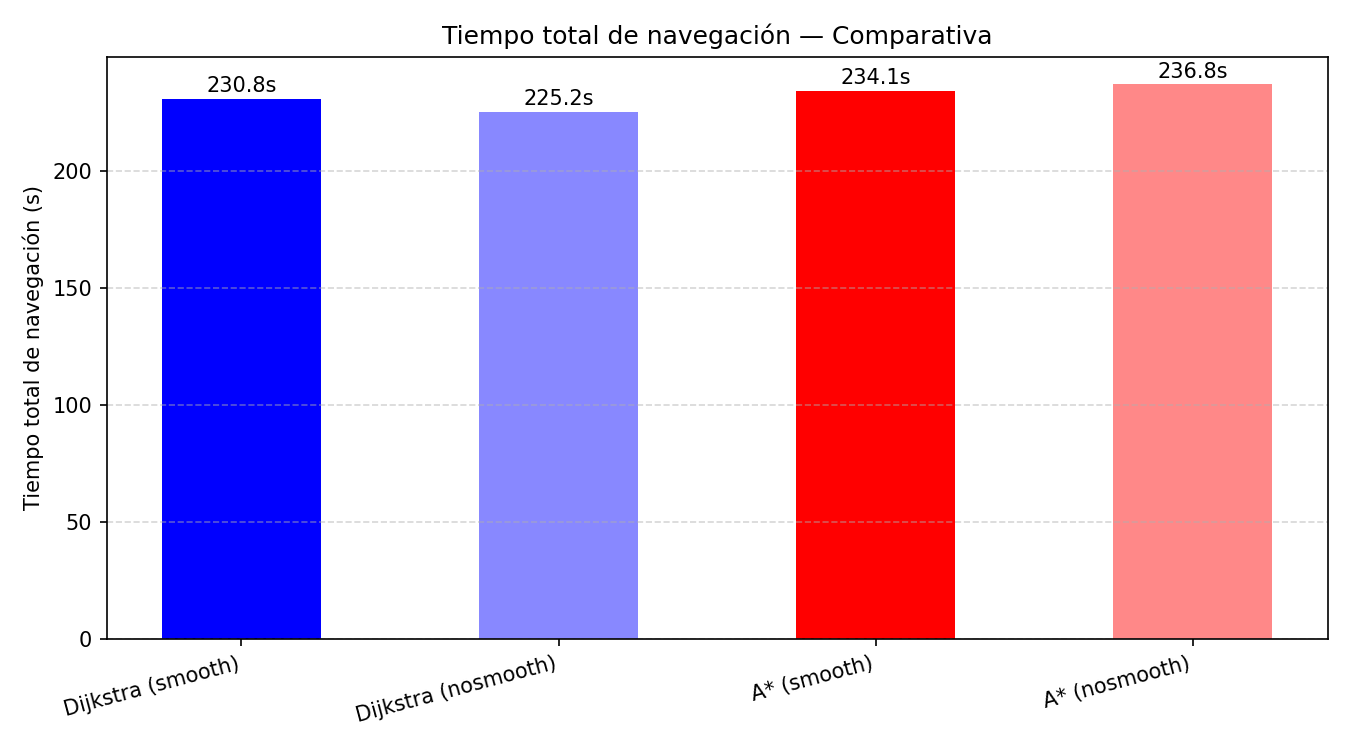
\includegraphics[width=0.75\textwidth]{figures/plots/dynamic/13_total_time}
    \caption{Tiempo total de navegación hasta \texttt{goal4\_compleja} — Comparativa.}
    \label{fig:total_time}
\end{figure}

Los tiempos totales de navegación son: Dijkstra nosmooth 225,2 s, Dijkstra smooth 230,8 s, A* smooth 234,1 s y A* nosmooth 236,8 s. La diferencia entre el más rápido y el más lento es de 11,6 s sobre un recorrido de aproximadamente cuatro minutos, lo que representa un 5\% de variación. Dado que cada configuración se ejecutó una única vez, esta diferencia debe interpretarse con cautela: parte de la variabilidad puede deberse a factores no controlados como la convergencia de AMCL o el estado inicial del costmap.

\subsection{Desviación respecto al plan}

Las figuras~\ref{fig:dev_dijkstra}--\ref{fig:dev_all} muestran la desviación del robot respecto a la trayectoria planificada a lo largo del tiempo, y la figura~\ref{fig:dev_mean} recoge la desviación media de cada configuración.

\begin{figure}[H]
    \centering
    \begin{minipage}{0.48\textwidth}
        \centering
        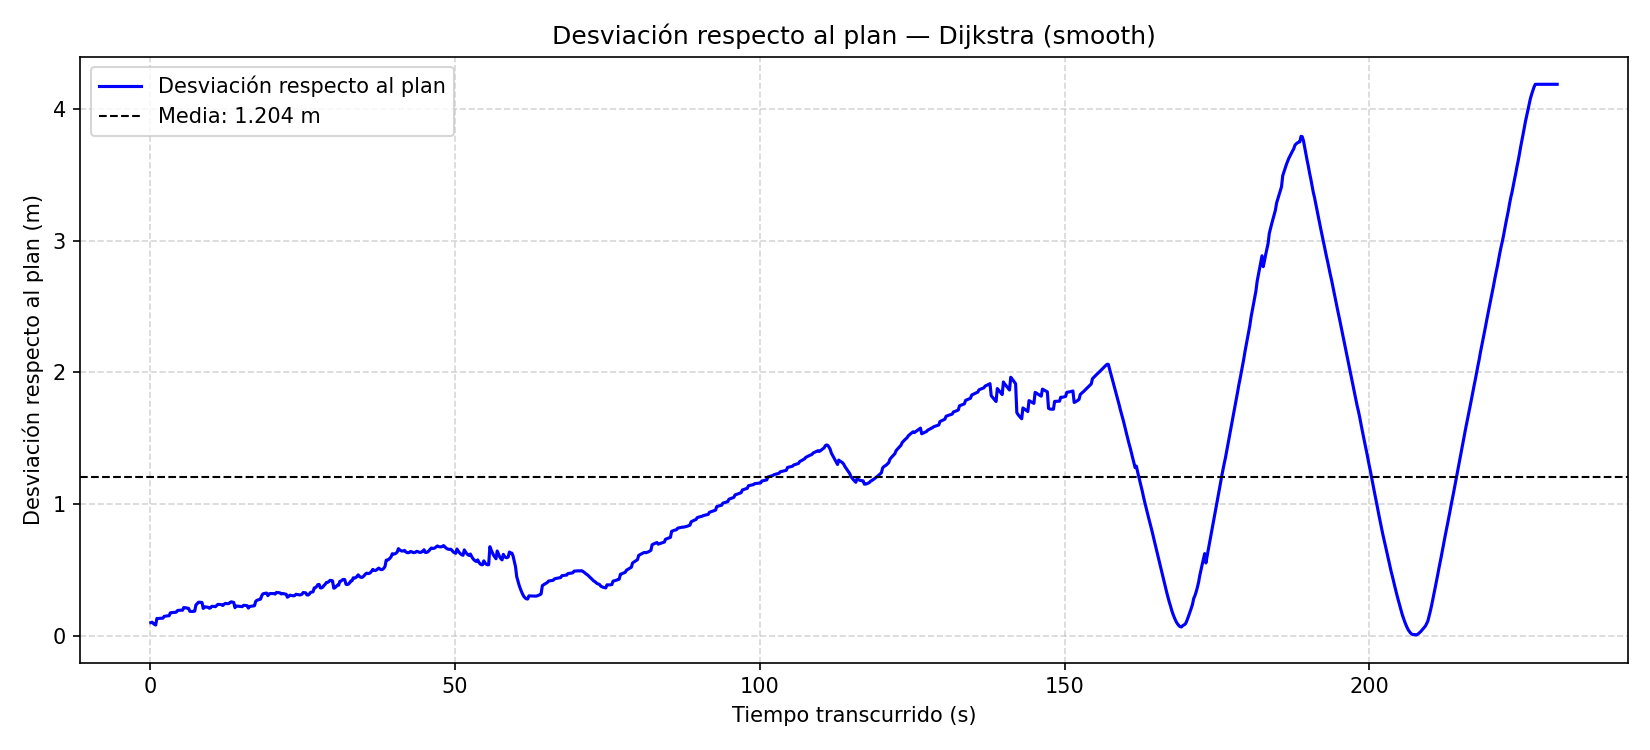
\includegraphics[width=\textwidth]{figures/plots/dynamic/15_deviation_dijkstra}
        \caption{Desviación respecto al plan — Dijkstra smooth.}
        \label{fig:dev_dijkstra}
    \end{minipage}
    \hfill
    \begin{minipage}{0.48\textwidth}
        \centering
        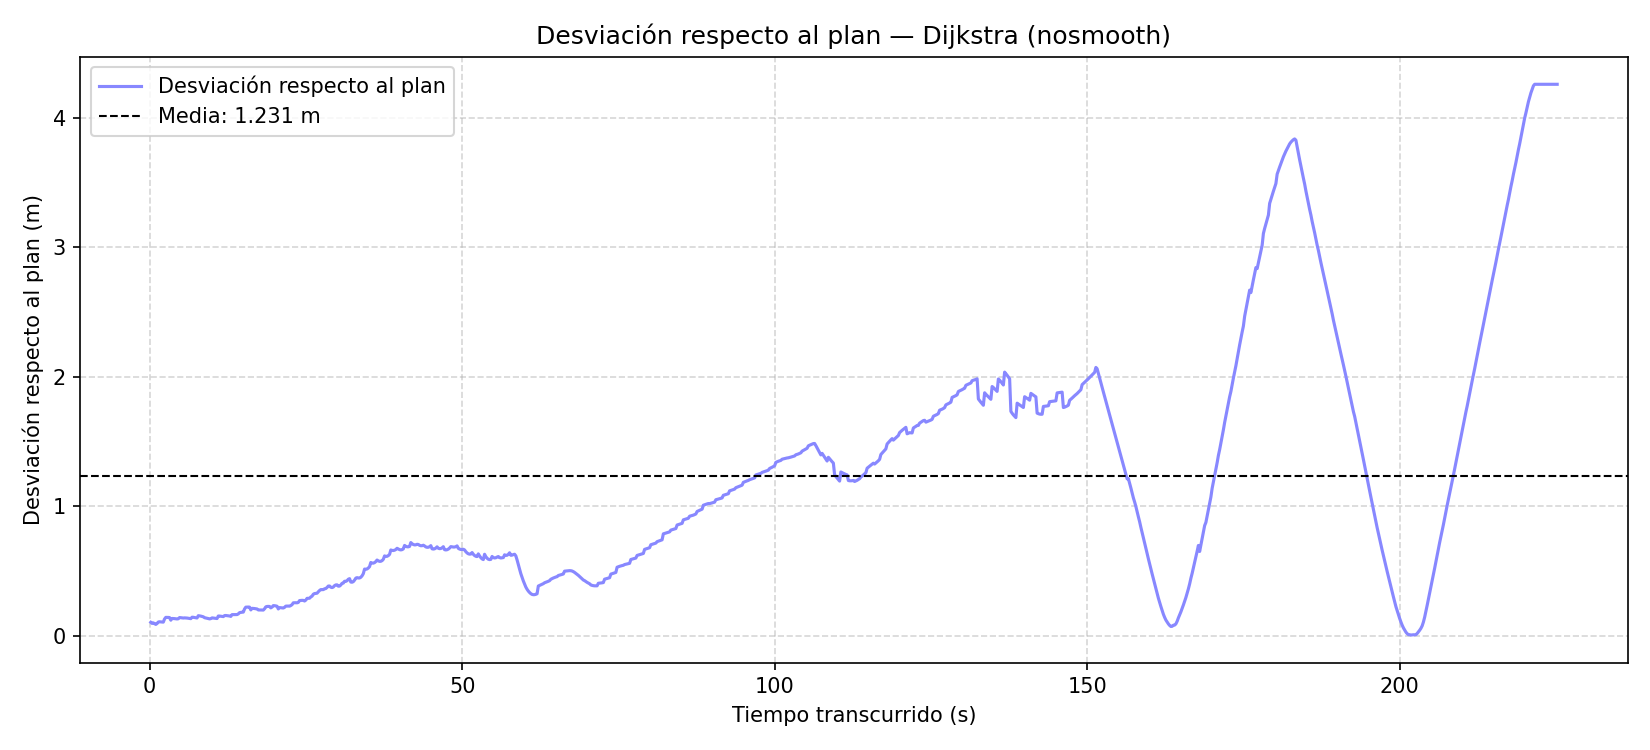
\includegraphics[width=\textwidth]{figures/plots/dynamic/16_deviation_dijkstra_nosmooth}
        \caption{Desviación respecto al plan — Dijkstra nosmooth.}
        \label{fig:dev_dijkstra_nosmooth}
    \end{minipage}
\end{figure}

\begin{figure}[H]
    \centering
    \begin{minipage}{0.48\textwidth}
        \centering
        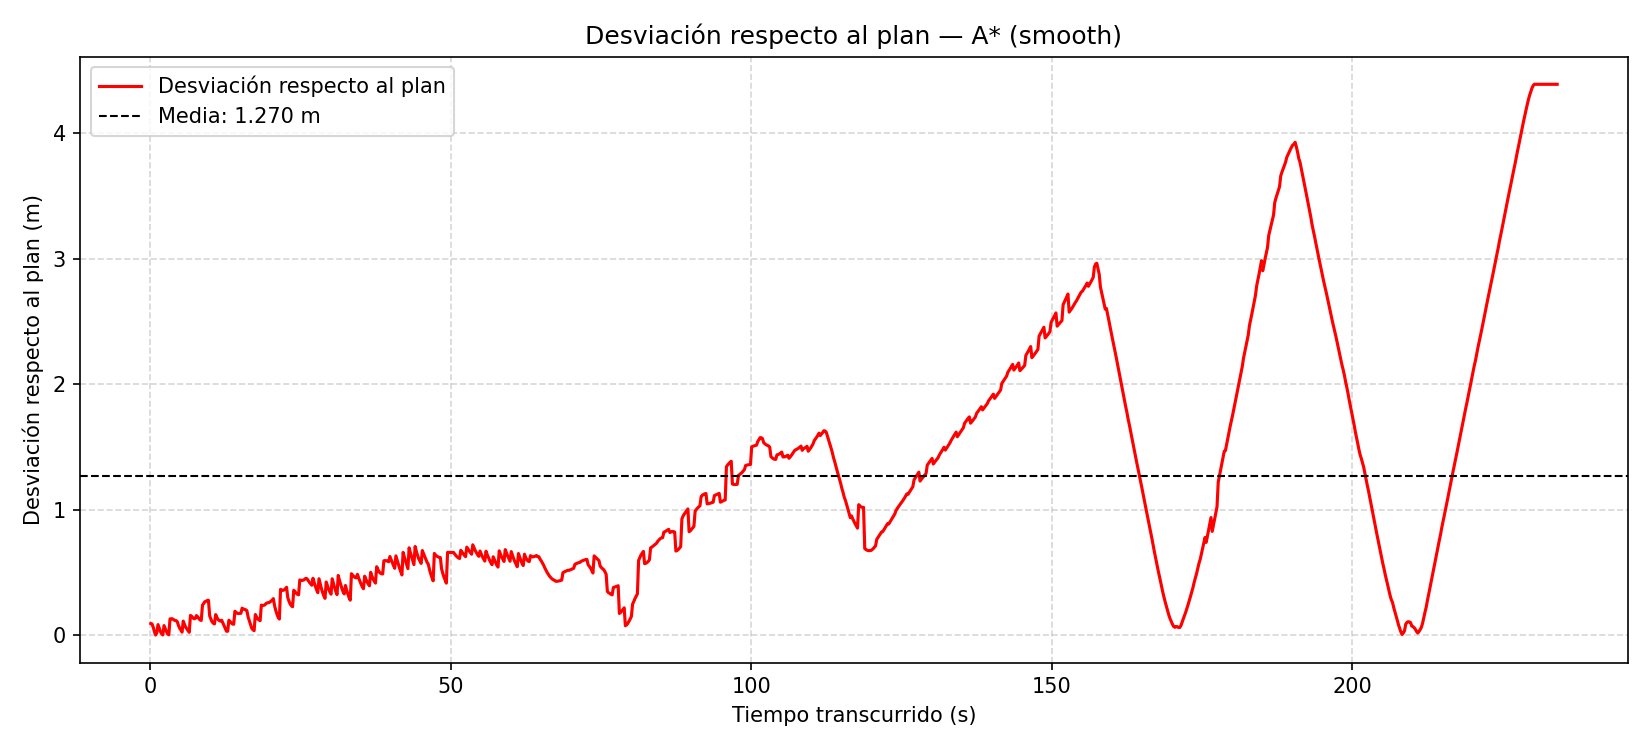
\includegraphics[width=\textwidth]{figures/plots/dynamic/17_deviation_astar}
        \caption{Desviación respecto al plan — A* smooth.}
        \label{fig:dev_astar}
    \end{minipage}
    \hfill
    \begin{minipage}{0.48\textwidth}
        \centering
        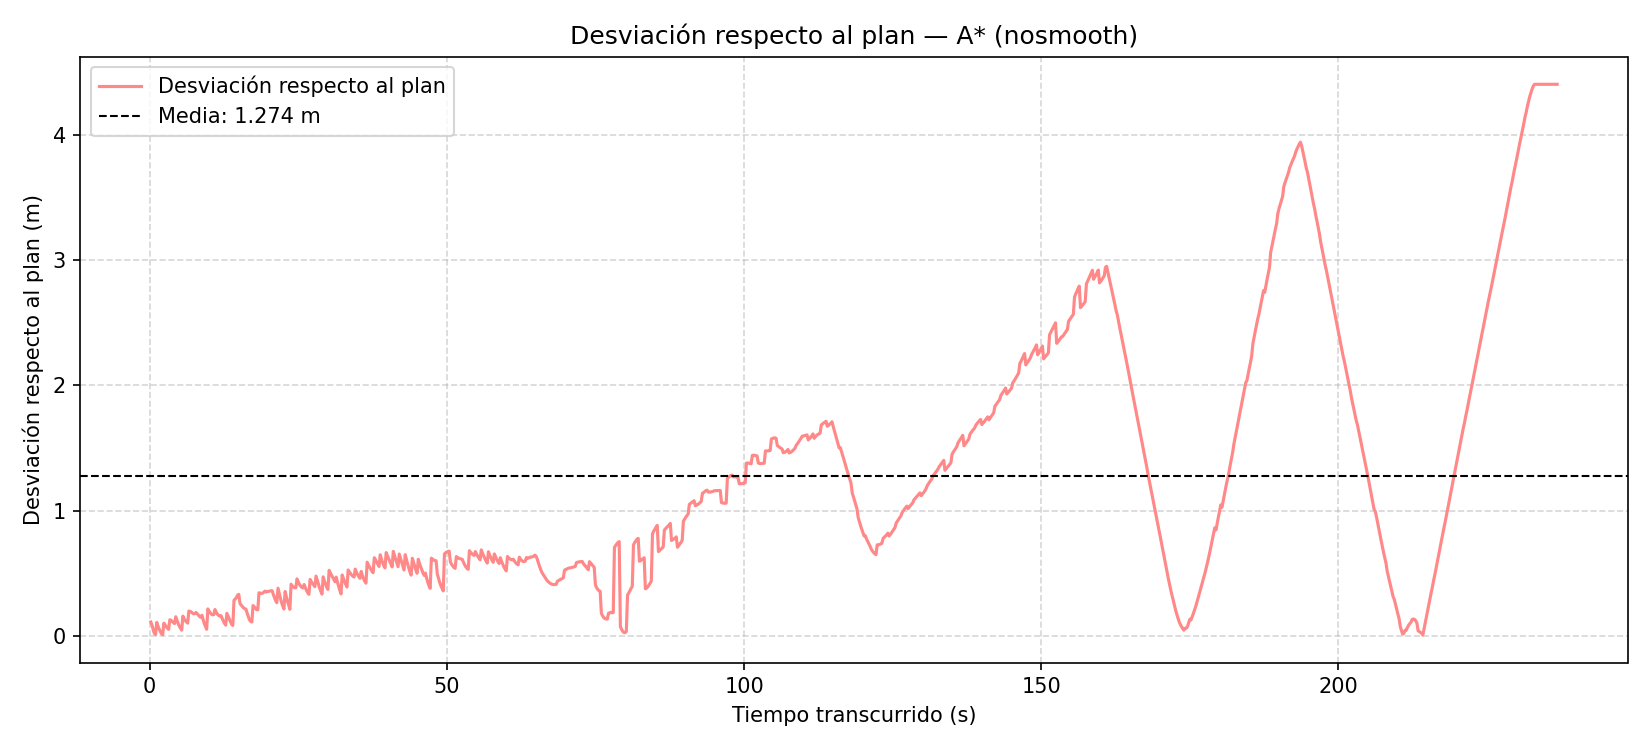
\includegraphics[width=\textwidth]{figures/plots/dynamic/18_deviation_astar_nosmooth}
        \caption{Desviación respecto al plan — A* nosmooth.}
        \label{fig:dev_astar_nosmooth}
    \end{minipage}
\end{figure}

\begin{figure}[H]
    \centering
    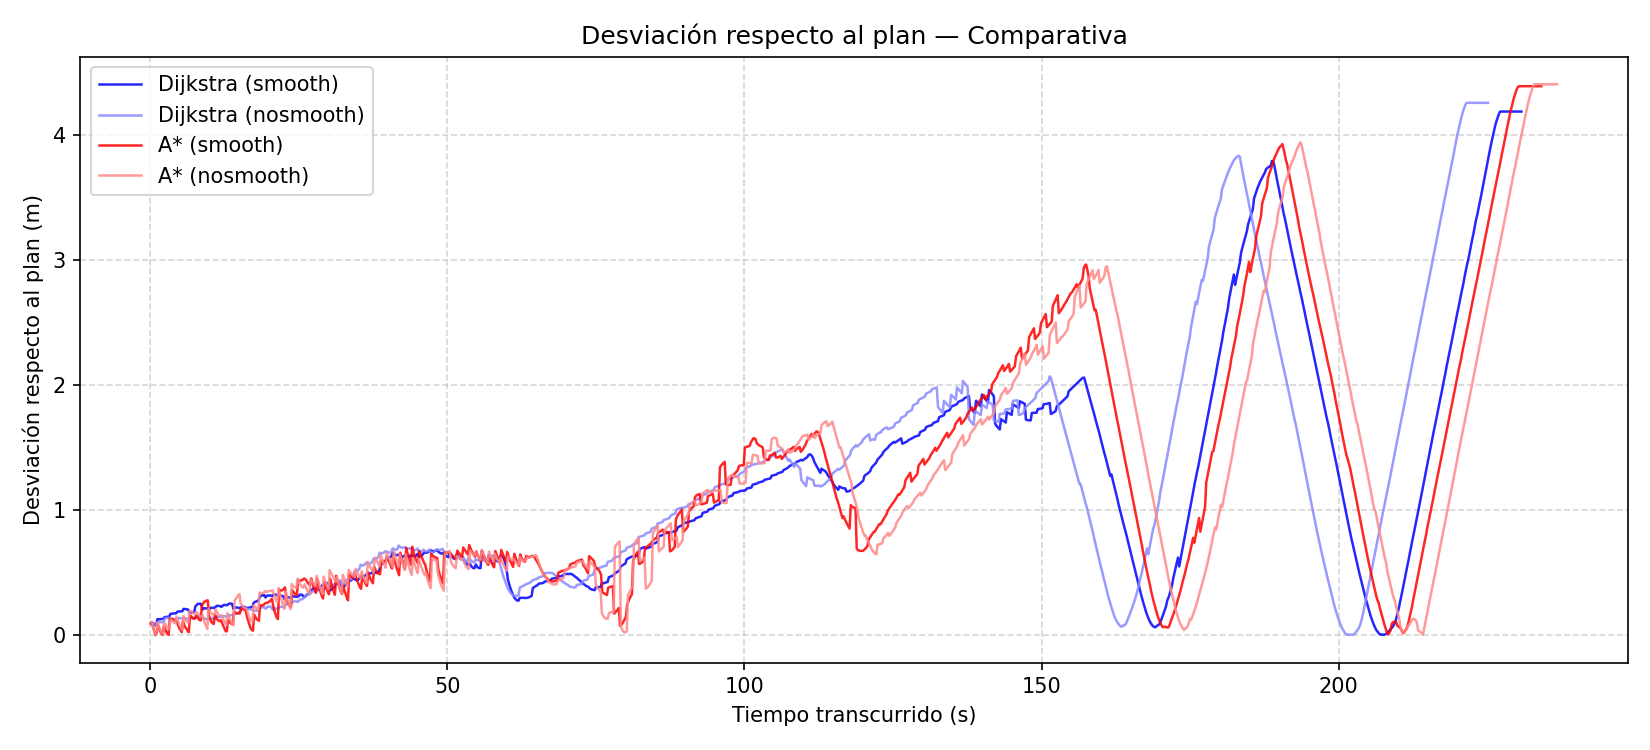
\includegraphics[width=0.9\textwidth]{figures/plots/dynamic/19_deviation_all}
    \caption{Desviación respecto al plan — Comparativa de las cuatro configuraciones.}
    \label{fig:dev_all}
\end{figure}

\begin{figure}[H]
    \centering
    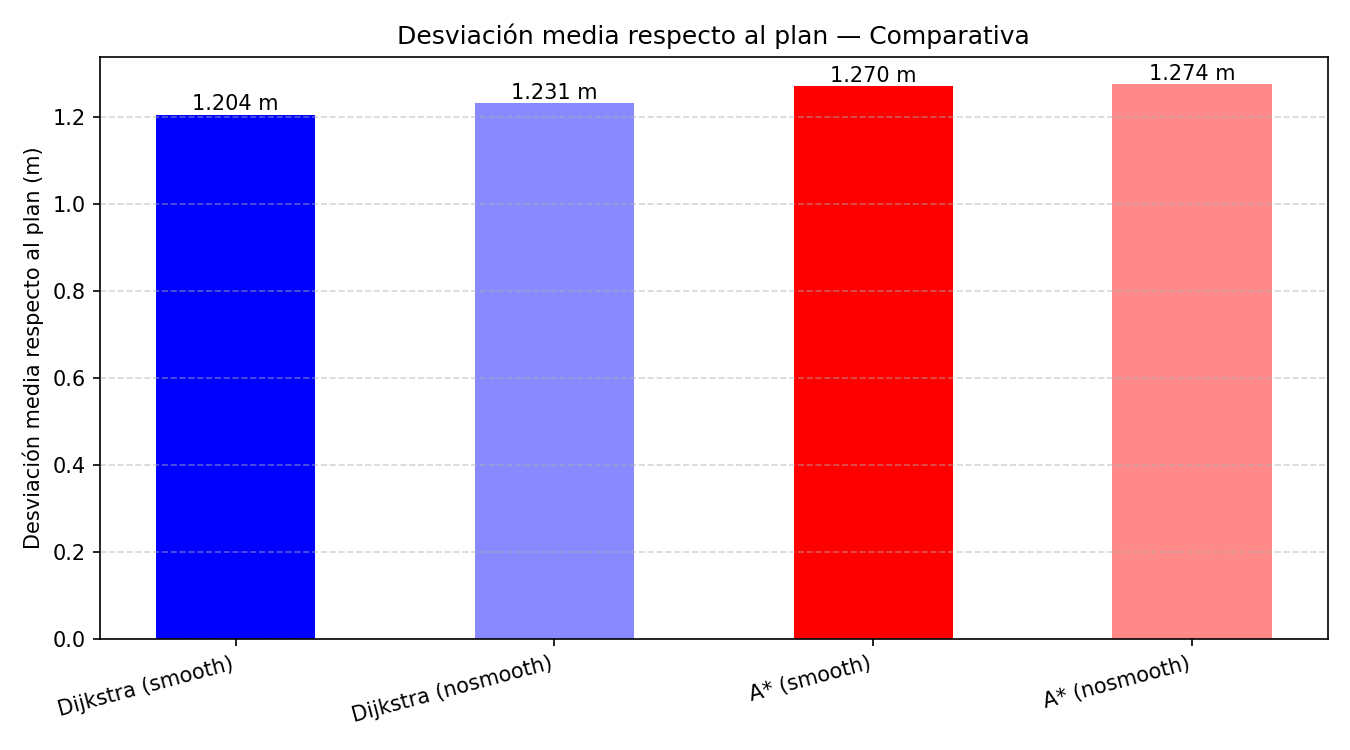
\includegraphics[width=0.75\textwidth]{figures/plots/dynamic/20_deviation_mean}
    \caption{Desviación media respecto al plan — Comparativa.}
    \label{fig:dev_mean}
\end{figure}

El perfil de desviación presenta la misma forma general en las cuatro configuraciones: desviación baja y creciente durante los primeros 150 s, seguida de oscilaciones de gran amplitud (picos de hasta ~4,2 m) en los últimos 80 s. Esta estructura refleja las dos fases de la trayectoria: la primera mitad, más abierta y con menos obstáculos, en la que el robot sigue el plan con relativa fidelidad; y la segunda mitad, con más restricciones geométricas, donde el robot se aleja y recupera el plan repetidamente mientras el controlador local gestiona los obstáculos.

La gráfica comparativa (figura~\ref{fig:dev_all}) muestra que las curvas de A* presentan más variabilidad en la fase inicial (0--150 s): las oscilaciones son más frecuentes y de mayor amplitud que en Dijkstra, lo que refleja los ajustes continuos de dirección que impone la trayectoria más irregular de A*. A partir de t=150 s, los cuatro algoritmos se comportan de forma similar, con picos y valles en las mismas posiciones temporales aproximadas.

En términos de desviación media (figura~\ref{fig:dev_mean}), Dijkstra smooth obtiene el mejor resultado con 1,204 m, seguido de Dijkstra nosmooth con 1,231 m, A* smooth con 1,270 m y A* nosmooth con 1,274 m. La diferencia entre el mejor y el peor es de 0,070 m, un valor modesto que ilustra cómo el controlador local DWB tiende a igualar el comportamiento de ejecución independientemente del planificador global. No obstante, la tendencia es consistente con el análisis estático: las configuraciones con menor irregularidad de trayectoria producen menor desviación media durante la ejecución.

\section{Discusión de resultados}

Los resultados obtenidos permiten extraer las siguientes conclusiones sobre el comportamiento de los algoritmos evaluados en el entorno de simulación utilizado:

\textbf{Dijkstra produce trayectorias significativamente más suaves que A* en NavFn:} La irregularidad de A* es entre 4 y 5 veces mayor que la de Dijkstra en el objetivo más complejo, y la curvatura media entre 3 y 5 veces mayor en los objetivos con obstáculos. Esta diferencia es estructural y no se corrige con el suavizado de NavFn.

\textbf{El suavizado tiene un efecto limitado sobre la irregularidad:} La reducción de irregularidad que aporta \texttt{do\_refinement: true} es inferior al 5\% en ambos algoritmos. Su efecto más apreciable es sobre la curvatura media, donde mejora entre un 10 y un 20\% en la mayoría de los objetivos. El suavizado tiene un coste en tiempo de planificación de entre 3 y 9 ms en Dijkstra.

\textbf{A* es más rápido en planificación pero a costa de mayor irregularidad:} A* nosmooth es consistentemente el más rápido en todos los objetivos, con tiempos de planificación entre un 20 y un 50\% menores que Dijkstra smooth. Sin embargo, las trayectorias que genera son marcadamente más irregulares, lo que se traduce en mayor velocidad angular durante la ejecución y mayor desviación media respecto al plan.

\textbf{Las diferencias en ejecución son reales pero moderadas:} El controlador local DWB absorbe parte de las diferencias entre planificadores: los tiempos totales de navegación difieren en apenas un 5\% y las desviaciones medias en menos de 0,1 m. La diferencia más visible en ejecución es el perfil de velocidad angular, que es notablemente más errático en A*.

\textbf{La limitación de una única ejecución por configuración condiciona las conclusiones:} Dado que cada experimento se realizó una única vez, los resultados individuales pueden verse afectados por factores no controlados. Las tendencias observadas son consistentes con el análisis estático, lo que refuerza su validez, pero una comparativa estadísticamente robusta requeriría múltiples ejecuciones por configuración.
